\documentclass[twoside,openright,12pt,a4paper,spanish]{book}
\evensidemargin 10pt
\oddsidemargin  70pt

\usepackage[utf8]{inputenc}
\usepackage[T1]{fontenc} 
\usepackage{fullpage}
\usepackage{graphicx}
\usepackage{amssymb}
\usepackage{amsmath}
\usepackage{amsfonts}
\usepackage{synttree}
\usepackage{enumerate}
\usepackage{tocloft}
\usepackage{color}
\usepackage{apacite} 
\usepackage[all]{xy}
\usepackage[spanish]{babel}
\linespread{1.1}
\title{\textbf{}}
\author{Alexander Adalid Castillo Romero}
\usepackage{multicol}
\usepackage{setspace}
\usepackage{url}

\setlength{\parindent}{0.5in}
\setlength{\parskip}{0mm}
\setcounter{secnumdepth}{4} 
\setcounter{tocdepth}{4} 

\renewcommand{\baselinestretch}{1.5}

\begin{document}

\begin{titlepage}
\begin{center}


\includegraphics[width=3.15 cm,height=3.75 cm]{unam.png} 

\normalsize{\textbf{UNIVERSIDAD NACIONAL AUTÓNOMA DE MÉXICO}\\
FACULTAD DE FILOSOFÍA Y LETRAS \\ \ \\ \ \\ \ }


\Large{UN ANÁLISIS FILOSÓFICO SOBRE LAS IMPLICACIONES DEL TEOREMA DE ZERMELO SOBRE EL AJEDREZ\\ \ \\ \ }

\normalsize{T E S I S\\
QUE PARA OPTAR POR EL TÍTULO DE\\
LICENCIADO EN FILOSOFÍA\\
$\ $\\


PRESENTA:\\
$\ $ \\
ALEXANDER ADALID CASTILLO ROMERO\\
$\ $ \\
$\ $ \\
\footnotesize{TUTOR: DR. CRISTIAN ALEJANDRO GUTIÉRREZ RAMÍREZ (FFyL-UNAM)}\\
$\ $ \\
$\ $ \\
CIUDAD UNIVERSITARIA, CIUDAD DE MÉXICO, MÉXICO   $\ \ \ \ $  ENERO $\ \ \ \ $ 2024
$\ $\\
}


\end{center}
\end{titlepage}

\newpage
$\ $
\thispagestyle{empty} % para que no se numere esta pagina

\chapter*{}
\pagenumbering{roman} % para comenzar la numeracion de paginas en numeros romanos
\begin{flushright}
\textit{A Mario y a Xochitl}
\end{flushright}

\newpage
$\ $
\thispagestyle{empty} % para que no se numere esta pagina

\chapter*{}
 
\begin{flushright}
\singlespacing
\textit{La belleza de un movimiento no se refleja en su apariencia, sino en el pensamiento que hay detrás de el.}

-Siegbert Tarrasch

\end{flushright}

\newpage
$\ $
\thispagestyle{empty} 


\chapter*{Agradecimientos}
\addcontentsline{toc}{chapter}{Agradecimientos} 
\markboth{AGRADECIMIENTOS}{AGRADECIMIENTOS} 

\noindent Construir los agradecimientos sobre este trabajo me ha sido más complicado de lo que esperaba, probablemente gracias a que la redacción de la tesis ha sido un proceso un poco largo y no consigo hacerme la idea de que finalmente lo hemos concluido. Para este punto no sabía si escribir algo satírico en los agradecimientos, algo ambiguo o simplemente no poner nada, para no pelearme por no saber que escribir. Finalmente he decidido simplemente tomarme un tiempo para dejarle un breve mensaje a algunas de las personas que me acompañaron a lo largo de este trabajo, ya que ciertamente no hubiera sido posible sin su apoyo. Gracias a todos ustedes:

A mis padres, Mario y Xochitl, por decidir ser los padres que son, por ser mejores de lo que el mundo esperaba de ustedes y por no ceder ante lo complicado que ha sido llegar a este punto. A mis hermanos, Alina, Alondra, Agustín y Luz, por hacerme sentir que no soy un tan mal ejemplo. Sin ustedes la última parte de este trabajo no hubiera sido posible. A Paulina, por tantas cosas que le he agradecido, que le agradezco y probablemente, que le agradeceré y aún así no será suficiente, por fin sacamos esto adelante. A Ricardo y Luis Romero, por incentivar y alimentar mi gusto por la lectura, la música, las ciencias y aquellas cosas sobre el mundo que vale la pena conocer. A Beto, Mary, Gabi, Edgar, Yamileth y Viviana, por su disposición a apoyarme cuando lo llegué a necesitar.

A Iván Niño, un gran amigo y gracias a quien comencé a disfrutar tanto del ajedrez, nunca terminaré de agradecerte las muchas oportunidades que me diste, una parte de este trabajo es gracias a ti. A Gabriel, por las traducciones, discusiones y la paciencia que tenia al esperar que terminara de hablar para decirme que no entendía. A Issac y Jacqueline, por la confianza en que en algún momento iba a poder terminar con este trabajo y su interés en que lo concluyera. A Armando Moto, por poner en duda mi concepción sobre amistad, más para bien que para mal y por hacer más amena la vida en ciencias, junto a Nath y Hazel. A Dennis, Fernanda, Santiago, Hector, Edu y Fer, por aguantar las partidas que perdimos porque yo estaba más concentrado escribiendo que holdeando mid.

A Cristian Gutierrez, por hacerme sentir más como un colega y no solo un alumno, por el increíble apoyo que recibí al escribir este trabajo, por las horas que invertiste a revisarme y corregirme, porque a pesar de los tropiezos del tiempo conseguimos terminar el proyecto. Espero que podamos seguir trabajando juntos. Al seminario de tesistas de Cristian, gracias Esperanza, Eduardo, Elena, Álvaro, Raymundo, Balam, Andrea, Fernanda, Abraham y todos los miembros, por leerme y dedicar su tiempo a ayudarme a pulir este trabajo. A Sam, por tomarse la molestia de explicarme sobre teoría de juegos aún cuando siempre que me hacía preguntas le respondía mal. A Hugo, Carlos, Ivan, Lourdes y JuanFe, a quienes admiro. Me da gusto haber llegado al final de la carrera y que fueran parte de ella. De igual modo gracias a Ernesto, Sonia, Grajales, Emelia y Rocío Sosa, por compartir la pasión que tienen por su labor, espero algún día poderme expresar como lo hicieron ustedes.

A mis gatos, Chispa, Minimí y El Gordo, por acompañarme, gritarme, rasguñar el monitor y apagarme la computadora durante tantas noches en las que de repente me llegaba alguna idea lúcida y me sentaba a escribir. A Overleaf, por no permitir que perdiera mi avance cuando mi gato dejaba su patita sobre el botón de encendido de la computadora y la apagaba. 

De nuevo, muchas gracias, espero que puedan ver reflejado el resultado de haber concluido con esta parte de mi carrera. \cite{sep-church-turing}

\begin{flushright}
    A.
\end{flushright}

\newpage
$\ $
\thispagestyle{empty} 

\tableofcontents % indice de contenidos

\chapter*{Introducción}

Escribir sobre el ajedrez en un aspecto que no sea propiamente del juego aunado a una perspectiva filosófica es algo complicado. Cuando empecé a generar esbozos sobre este trabajo mis ideas giraban en torno a tratar de describir de manera rigurosa una estética del juego. Desarrollar un trabajo de ese tipo me parecía más fácil de evidenciar como filosófico que uno sobre la lógica o su aspecto matemático. Discutí esta primera cuestión con mi asesor y me explicó lo complicada que sería esa tarea y me sugirió intentar abordar el ajedrez desde otra perspectiva. 

El interés que ambos teníamos sobre el juego y que yo haya dedicado unos cuantos años a disfrutarlo en su aspecto lúdico nos llevaron poco a poco a investigar tanto sobre jugadores, como sobre torneos hasta que poco a poco profundizamos en los aspectos mas teóricos del juego.
Eventualmente llegamos al teorema de Zermelo, que para cuando menos cuenta me había dado, ya representaba el núcleo del trabajo que estamos escribiendo. Gracias a ello, pudimos fijar un punto de partida para el trabajo: Tratar de observar las consecuencias de dicho teorema sobre el ajedrez, particularmente su impacto en la práctica del juego.

Para abordar esta discusión, el primer capitulo de este trabajo versa sobre Zermelo, comenzando en un aspecto hist\'orico donde se rescatan cuestiones relevantes alrededor del momento en el que se escribi\'o el teorema, as\'i como un par de perspectivas ajenas sobre el teorema y su relaci\'on con fen\'omenos m\'as recientes, como la teor\'ia de juegos. El siguiente paso es la reconstrucci\'on de la prueba, que ya despu\'es de haberla trabajado se trat\'o de sintetizar y con ello volver m\'as accesible su lectura. Finalmente, el cap\'itulo cierra con un esfuerzo por acotar el teorema al caso particular del ajedrez. Esta secci\'on surge gracias a mi afici\'on personal, pues hab\'ian algunas cuestiones sobre el teorema de Zermelo que considero podr\'ian ser m\'as claras si se muestran desde un caso particular, tales como la finitud del juego o c\'omo funciona la exclusi\'on de repeticiones.

Una realidad es que la práctica y el estudio del ajedrez dista mucho del análisis que presentaba Zermelo, además de que abordar la práctica de un deporte particular no parece muy filosófico, al menos en principio. Mientras que con Zermelo se habla de conjuntos, secuencias y posiciones particulares, el ajedrez que yo conocía era en términos de aperturas, medio juego, finales y teoría. Esto nos permitió tratar de buscar la relación que surgía entre el proceso descrito en el teorema y lo que hacemos las personas cuando jugamos ajedrez. Parece necesario entonces desarrollar c\'omo es que funciona el teorema de Zermelo en la pr\'actica y con ello empezar a contrastar al ajedrez con otros juegos cuyo resultado ya se conoce. Sobre esto versa el segundo cap\'itulo. 

Conociendo el resultado del teorema podemos observar que el ajedrez se puede resolver y que ya hacemos este proceso a una menor escala con los problemas es pertinente preguntarse por qué no se ha aplicado el teorema al ajedrez para encontrar la secuencia óptima y el resultado. La respuesta que pretendo ofrecer es que dada la cantidad posiciones y partidas que hay en el ajedrez, analizarlas mediante el proceso de Zermelo sería una tarea tan larga que parece no haber tiempo suficiente en esta vida para resolverlo. Mi respaldo para ello son 2 sistemas similares en características al ajedrez: Las damas inglesas y el juego de gato\footnote{Que tambi\'en tiene otros nombres, como tic tac toe, sitauci\'on que desconoc\'ia.}.

Ambos sistemas son regidos por el teorema y, mientras que parece que el juego de gato se puede resolver de manera intuitiva y hasta geom\'etrica, el proceso para las damas inglesas requiri\'o años para su resolución, e incluso se considera que no es una resolución fuerte del juego. Gracias a mostrar que el proceso de búsqueda de una estrategia varía entre sistemas, se puede exhibir al ajedrez y como los humanos pueden resolver problemas frente a lo extenso que puede resultar intentar obtener la estrategia óptima sin que se posea una heurística para restringir las posiciones a calcular. Mientras que para el gato el proceso se hizo por fuerza bruta y se obtienen todas las secuencias, el resolver las damas y el ajedrez funciona de manera muy distinta. Estos dos capítulos constituyen un análisis lógico-filosófico --particularmente desde la teoría de conjuntos-- sobre el ajedrez y las consecuencias de intentar obtener más resultados sobre él a partir del teorema de Zermelo.

El tercer capítulo se desarrolló para exponer de manera más clara cómo es que este trabajo es un análisis filosófico y exponer un punto adicional: incluso si el ajedrez no es un fenómeno filosóficamente relevante desde la perspectiva de la lógica, lo puede ser desde otras disciplinas. Para ello, me justifico en tres perspectivas distintas: la epistemología, la estética y la ética-política. Estas tres perspectivas ofrecen un acercamiento distinto al ajedrez que va desde las problemáticas que surgen de usarlo como comparativa intelectual entre humanos y máquinas, además de la diferencia de juego que puede existir entre ambos, pasando por cómo se puede constituir una estética del juego en comparación con las matemáticas y algunas de sus características, para finalizar con la presentación del juego en su aspecto competitivo, como fenómeno cultural y las consecuencias políticas que han surgido a través de él.

En conjunto, este trabajo presenta un análisis del ajedrez, principalmente enfocado en la lógica como área de la filosofía. De manera intuitiva no parece evidente cómo es que un juego de mesa --siendo benevolentes incluso podemos llamarle deporte-- puede detonar una discusión de carácter filosófico, pero la exposición a través de la perspectiva de Zermelo permite abordar tanto al ajedrez como el alcance de la teoría de conjuntos. Aunado a ello, existen diversas alternativas de estudio producto de la complejidad del juego, como su aspecto deportivo o intelectual que pueden generar sus propios análisis.


\addcontentsline{toc}{chapter}{Introducción}

\markboth{Introducción}{Introducción}


\chapter{El teorema de Zermelo}
\pagenumbering{arabic}
\setcounter{page}{1}
\markboth{Capítulo}{ }

\section{Introducción}

\noindent Este primer capitulo tiene la intención de abrir el camino para la aplicación del teorema de Zermelo sobre el ajedrez, esto a través de 3 puntos importantes, cada uno desarrollado en una sección.
El primero de ellos es conocer un panorama general de la publicación del teorema junto con un acercamiento a la vida de Ernst Zermelo, que si bien sera breve, ayuda a mostrar porque se le toma relevancia al teorema de manera bastante póstuma a su publicación, además de presentar un par de perspectivas ajenas sobre el teorema y lo fuerte que puede llegar a ser. Esta sección (1.2) está fundamentada básicamente en los textos \emph{Collected Works} \cite{zermelo2010ernst} y el artículo \emph{Zermelo and the early history of game theory} \cite{schwalbe2001zermelo}.

El segundo (sección 1.3) es una reconstrucción de la prueba del teorema de Zermelo. Esta se realizó con la intención de volver más accesible el teorema al lector dados 3 problemas particulares. El primero es la maquinaria conjuntista de la demostración, pues los símbolos y la redacción en prosa no suelen dar claridad de manera inmediata. El segundo es el idioma, pues la prueba original se escribió en alemán y las traducciones que fueron encontradas para esta investigación se encontraban en inglés. El tercero es que gracias a que la tesis versa sobre las aplicaciones del teorema al ajedrez, reconstruir la prueba permite exhibir de manera más clara elementos tales como las cotas sobre los conjuntos que construye Zermelo, para más adelante, cuando se aborde la aplicación del teorema al ajedrez, resulte evidente cómo son estos conjuntos y cómo es que se limitan.

El tercer punto consiste en aclarar ciertos aspectos del teorema que Zermelo da por hecho -como que el juego es finito-- o aquellos que simplemente no aparecen en la prueba original, pero salen a la luz cuando se observa con detenimiento el caso del ajedrez --como los problemas al definir una cota--. Además se incluye un acercamiento a ciertas reglas particulares del juego que ofrecen maneras de interpretar elementos de la prueba original --como la concepción de \textit{no perder} o \textit{empatar}--.

De manera general, se espera que al finalizar el capitulo se tenga: tanto un panorama general del contexto de la publicación del teorema como de la vida de Ernst Zermelo en ese entonces, una comprensión de la prueba original a través de una reconstrucción que resulte mas fácil enfocar al ajedrez y un acercamiento a los problemas que surgen al observar el teorema desde un sistema particular.

\section{Contexto del teorema}

\noindent Ernst Zermelo (1871-1953) fue un matemático dedicado a la teoría de conjuntos y pionero en lo que actualmente se conoce como \emph{teoría de juegos}. Algunos de sus trabajos más importantes fueron su introducción al axioma de elección en 1904 y la axiomatización de la teoría de conjuntos en 1908, que resultaron relevantes para el enriquecimiento de las matemáticas y el desarrollo de la teoría de conjuntos posterior a Cantor. Previo a su trabajo en Zurich se encontraba en Göttingen estudiando, tiempo donde coincidió con Planck, siendo su ayudante y con Hilbert, quien fue su profesor y eventualmente el director de su tesis doctoral.

Durante el periodo de 1910 a 1916 se encontraba trabajando en Zurich, en lo que se puede considerar el periodo más próspero de su vida, probablemente gracias a que fue pagado como profesor de universidad \cite{zermelo2010ernst}. Previo a la publicación del teorema se encontraba laborando como profesor de matemáticas impartiendo un curso de Cálculo Diferencial e Integral, además de uno de Ecuaciones Diferenciales, esto gracias al apoyo de Erhard Schimdt para sucederle como profesor, pues la buena respuesta por parte de Hilbert como asesor de su tesis doctoral motivó un consenso para que Zermelo tomara el lugar de Schmidt en una votación de 15 a 1 a su favor. Para 1912 Se encontraba pasando por una etapa crítica, pues había enfermado de tuberculosis, lo que lo motivó a considerar la publicación de sus obras o \textit{Collected Works}. Dado que el teorema es de 1913, este surge mientras Zermelo atravesaba una profunda depresión aunada a su enfermedad, que le acompañaría durante varios años más, hasta que fue retirado de la universidad de manera temporal debido a su afección.\footnote{Hay muchos aspectos que se pueden revisar de la vida de Zermelo disponibles en el texto \textit{Ernst Zermelo - Collected Works}}

El teorema de Zermelo\footnote{Llamarle \textit{El teorema de Zermelo} no es solo porque sea el único teorema suyo abordado en el texto, sino porque así se le conoce de manera general.} fue publicado en Alemania bajo el título \textit{Über eine Anwengdung der Mengenlehre auf die Theorie des Schachspiels} y a pesar de que el teorema es propiamente de teoría de conjuntos y sus aplicaciones, se considera es el primer paso en lo que actualmente se conoce como \textit{teoría de juegos}. La publicación del teorema pareció no tener una repercusión fuerte sobre el ajedrez, y ciertamente para ningún área, al menos en los primeros años. Kálmar y Köning pusieron en discusión el teorema y diversas cuestiones alrededor de él. Por una parte Köning -13 años después de la publicación original- se aventuró a realizar una generalización del teorema de Zermelo para juegos con números infinitos de posiciones, pero a las que se podía llegar a través de un numero finito de secuencias.

Además, argumentó que el trabajo de Zermelo estaba incompleto por dos razones; primero, que Zermelo falla en probar que si blancas se encuentra en una posición ganadora es siempre capaz de forzar una victoria en un numero de movimientos menor a la totalidad de posiciones en el juego, que fue una confusión en la interpretación sobre el comportamiento de negras respecto al juego, situación que puede considerarse debatible y se discutirá en un capitulo posterior del presente trabajo. La segunda razón fue un error de lectura por parte de Köning, pues omitió la consideración de que el mismo conjunto de piezas en el tablero puede representar dos (o más) estadios en el juego dependiendo de quién sea el turno.

Por otra parte Kálmar se metió a la discusión cuestionando si Zermelo había excluido la repetición en sus juegos, pues parece que este no demuestra de manera formal que esta debe quedar excluida de las \textit{posiciones ganadoras} lo que lo motiva a realizar una generalización ahora no solo del trabajo de Zermelo, sino también de la reciente publicación de Köning respecto a este, partiendo de si realmente existía una cota superior. De manera general, el trabajo de ambos sobre el teorema de Zermelo versa en encontrar si en un juego de ciertas características es posible encontrar una cota superior para posición ganadora o de encontrarse en una posición perdedora, cuánto es posible retrasar la derrota. 

El trabajo de Köning y Kálmar está sintetizado en un artículo titulado \textit{Zermelo and the early history of game theory} \cite{schwalbe2001zermelo}, junto con otras  afirmaciones sobre el teorema, por ejemplo, que el teorema muestra que el ajedrez está determinado \cite[p. 1]{aumann2019lectures}, mientras que otros proponen afirmaciones más fuertes, como que el teorema muestra que blancas -o el jugador que mueve primero- no puede perder, aunque no sea clara la estrategia bajo la cual este pueda ganar \cite[p. 107]{dimand1996history}, e incluso se llega a hablar sobre una inducción \textit{hacía atrás} \cite[p. 32]{binmore1994teoria} o \textit{retroinducción} como se usará a lo largo de este texto.

El hecho de que todas estas propuestas sobre lo que dice Zermelo sean tantos años posteriores a la publicación original sugieren que el fenómeno que aborda era novedoso para la época. Zermelo acota su teoría a sistemas de características particulares; juegos finitos de información perfecta que poseen un equilibrio de Nash de estrategia pura \cite[p. 272]{mas1995microeconomic}. Tómese en cuenta que el concepto de equilibrio de Nash\footnote{El equilibrio de Nash propone que en todo juego existe al menos una estrategia \'optima para ambos jugadores, o, en términos de teoría de juegos, una estrategia que maximiza la función de pago o de utilidad de cada jugador \cite{de2014equilibrio}.} nace hasta la década de 1950, lo que parecería evidencia de que Zermelo trabajaba sobre algo adelantado a su tiempo.

El teorema fue tomando relevancia hasta convertirse en la base de la teoría de juegos contemporánea. La aplicación de la teoría de conjuntos ya no quedaba solo en el estudio de juegos (en el sentido más mundano de la palabra) o si son determinados o que tan largos pueden ser, sino que la propuesta de Zermelo abre paso a analizar una cantidad enorme de situaciones si éstas pueden ser planteadas de manera similar a la generalización del ajedrez, un sistema de dos personas, con exclusión de suerte e información completa, pero sin agotarse ahí.

A partir del teorema se pueden decir muchas cosas sobre los juegos\footnote{Juegos no en un sentido coloquial, sino como sistemas.}, pero ¿qué tanto se puede decir sobre el ajedrez? Ya se han hecho afirmaciones respecto a este caso particular, pero la evolución del ajedrez a lo largo del tiempo ha mostrado que el teorema de Zermelo puede abrir diferentes lineas de análisis, pues la complejidad del juego no permite que el teorema arroje resultados que banalicen el juego o modifiquen sustancialmente la práctica\footnote{Aunque quizá si el entrenamiento.}. El ajedrez es un caso particular que se puede explorar analizando la demostración original y cómo es que ésta queda acotada (o no) al juego.

\section{Reconstrucción de la prueba}
\noindent Para la reconstrucción de la prueba parece conveniente dividir en 4 secciones el Teorema de Zermelo \citeyear{zermelo1913anwendung}: La primera es la introducción, que incluye la justificación para el teorema así como la mención de los problemas de ajedrez, que resultarán relevantes a lo largo del análisis posterior. La segunda, centrada en el análisis de los conjuntos \emph{Ur(q)} y \emph{U(q)}, colecciones de finales en los que blancas llega a una posición ganadora a partir de una posición q dada. La tercera se encuentra centrada en las condiciones y consecuencias de que \emph{U(q)} sea vacío y la construcción del conjunto \emph{Vs(q)}, en el cuál blancas no pierde después de la posición s, lo que garantiza por lo menos tablas\footnote{Tablas es otra manera de referirse al empate en el ajedrez.} para blancas. La última parte se centra en hacer la analogía de \emph{Ur(q)} para negras y las conclusiones que Zermelo obtiene al aplicar el teorema al ajedrez.

Zermelo se centrará en el análisis de juegos como el ajedrez (aquellos que contemporáneamente definiremos como de dos participantes, suma cero, sin azar y con información completa). El punto de partida del teorema es la pregunta sobre si dada una posición arbitraria en alguno de estos juegos, esta puede ser evaluada de manera matemática y objetiva, para determinar si existe una estrategia que nos permita ganar (o no perder) sin importar cómo juegue el oponente. Ofrece un ejemplo de situaciones en las que de hecho ya existe este tipo de evaluación, los “problemas de ajedrez” que suelen ser posiciones en el tablero para las cuáles ya está especificado el resultado y el número máximo de movimientos en el que este sucede\footnote{Se da el número máximo ya que se trabaja bajo la idea de que el oponente va a intentar retrasar la derrota lo más que se pueda, y esta situación tiene más sentido cuando se conocen algunas implicaciones en la práctica de esto.}. 

Los problemas de ajedrez son una gran herramienta para mostrar cómo se visualizan los conjuntos que Zermelo utiliza en su prueba. Los juegos desde la maquinaria conjuntista utilizada en la demostración son secuencias de posiciones a partir del estadio inicial del sistema siguiendo las reglas particulares del juego. Estas se pueden agrupar en conjuntos con diversas propiedades, como tener una cardinalidad en particular, tener un primer elemento en común, etc. Gracias a esto Zermelo puede presentar tanto a los problemas de ajedrez como a lo que entiende como finales en términos de conjuntos de secuencias con propiedades particulares, tales como que o gana blancas, o blancas no pierde o gana negras. 

Continuando con la prueba, Zermelo menciona que dada la cantidad de recuadros en el tablero y de piezas movibles existe una cantidad finita de posibles posiciones dentro del juego. En cuyo caso se habla de un conjunto \textbf{P} de estadios del tablero de cardinalidad finita. Esta es la primer idea dentro de la prueba que Zermelo da por hecha sin probarla de manera formal, pero puede ser resuelta a través de cálculo combinatorio\footnote{Una formula que modela esto es presentada en una sección posterior.}.

Dentro del análisis se presenta la concepción de “finales” los cuáles son posiciones del tablero en las que se puede calcular cuál será el desenlace del juego por medio de una evaluación\footnote{La concepción de Zermelo sobre los finales no es la misma que la que se usa en la práctica, pero esto se detallará más adelante.}. Se utiliza a los finales gracias a que suelen ser posiciones en el tablero con una cantidad reducida de piezas, lo que facilita la evaluación. Zermelo menciona que hay solo dos maneras de terminar el juego: o en un jaque mate o en un empate. Cabe señalar que el empate tiene dos variantes: una en la que las posiciones del tablero son tantas que eventualmente se repetirían y otra en la que se llega a un punto en el que no existe una jugada legal con la cual dar seguimiento a una siguiente posición. Si bien Zermelo no la aborda del mismo modo que la primera, cumple las mismas condiciones que comprende el conjunto de finales en el que existe un empate\footnote{Presentar las diferentes maneras en las que se puede conseguir un empate puede ser útil para ver de manera más clara los limites de posiciones en el conjunto \emph{Vs(q)}, pero no es relevante en la determinación del resultado tanto del juego como de la prueba.}. 

En la segunda sección Zermelo presenta y describe al conjunto \emph{Ur(q)}; que contiene a las posibles posiciones q\footnote{q representa a una posición en el tablero, no necesita ser considerada como final y tampoco tiene una particularidad distinta, solo es parte de la secuencia.} a partir de un final \textbf{q} dado en el que blancas puede ganar en a lo más r movimientos. Cuando se habla de un final \textbf{q} como conjunto de posiciones, este no contiene todos los estadios del tablero posibles, sino que contiene una secuencia cambios de estadio (o movimientos) siguiendo las reglas particulares del juego, es decir, las piezas se mueven de una manera determinada y los movimientos son alternados, uno de negras y uno de blancas. La notación parece poco caritativa, pero en principio hay que rescatar las dos características que son condición necesaria para que de estar en el final q\footnote{q representa a un conjunto de posiciones q a partir de una posición particular a la que denomina final.}, este pertenezca a \emph{Ur(q)} y blancas se encuentre en una posición ganadora, es decir, en una posición a partir de la cual no importa la respuesta de negras, blancas cuenta siempre con una estrategia para forzar una victoria.

La primera es que: blancas gana en a lo más $r$ movimientos -suponiendo que el oponente juegue de manera óptima- por lo que entonces los elementos del conjunto \emph{Ur(q)} tendrían en total una cantidad de a lo más $r + 1$ de posiciones contando q, donde $r$ es la cantidad de cambios de estadios a partir de la posición inicial siguiendo las reglas particulares del juego y la suma representa la posición inicial. Como se sabe que la cantidad de estadios posibles del tablero es finita, este subconjunto sería también de cardinalidad finita, pues tampoco hay repetición de posiciones (más adelante se explica por qué). Si sucede que el oponente no juega de manera óptima, blancas ganaría en la misma cantidad de r movimientos o menos. Si gana en menos se sigue cumpliendo que gana en a lo más $r$ movimientos y se satisface la condición.

La segunda condición es que: Dado un final \textbf{q} = (q1, q2, q3, …) si en algún momento negras realiza un movimiento que no vaya de acuerdo con las posiciones q consideradas dentro del final \textbf{q}, blancas cuenta con una respuesta con la que continúa ganando en a lo más $r$ movimientos. Es decir, si negras juega una posición q’ blancas cuenta con una respuesta a q’ que cambia la secuencia contenida en \textbf{q}, pero si este final está contenido en \emph{Ur(q)}, blancas aún puede forzar una victoria. Esta consideración pondría en cuestión si negras está jugando de la mejor manera posible\footnote{Jugar de manera óptima implica que si negras se encuentra en una posición perdedora debe retrasar tanto como sea posible la derrota, al menos para efectos de esta demostración.}, por lo que incluso podría mencionarse que, si negras decide jugar a alguna posición q’ no contenida en la secuencia \textbf{q}, sería incluso más probable que blancas pueda terminar en una victoria con una cantidad menor de movimientos.

Estas dos características son condición necesaria para que un conjunto \emph{Ur(q)} exista y garantice que dada una posición q blancas se encuentre en una posición ganadora. Por supuesto si este conjunto \emph{Ur(q)} no es único, la unión de todos los conjuntos $\overline{U}$\emph{r(q)} posee también las mismas características. Si este conjunto no es vacío entonces blancas puede forzar una victoria en a lo más $r$ movimientos. En caso de que este conjunto sea vacío solo se garantiza que blancas no puede forzar una victoria, pero que blancas no gane no implica necesariamente que pierda (o que negras gane).

Posteriormente, Zermelo se centra en delimitar el conjunto \emph{Ur(q)} a través de una cota superior y una cota inferior para dar paso al conjunto que contiene a los finales en los que blancas no pierde después de cierta cantidad de movimientos. Es necesario precisar que quedarán excluidos -al menos por ahora- ciertas precisiones sobre las intersecciones entre los conjuntos que contienen la menor y mayor cantidad de movimientos necesarios para que blancas gane, esto en virtud de entender de mejor manera las cotas y como es que estas preservan la cantidad finita de posiciones posibles.

La cota inferior se denomina $ \rho $. Zermelo propone que existe un subconjunto dentro de \emph{Ur(q)} que contiene una cantidad \emph{r} = $ \rho $ de posiciones a partir q y esta es la cantidad mínima necesaria de movimientos para que blancas pueda forzar una victoria. Es importante considerar si el oponente se encuentra jugando de manera óptima, pues en caso de hacerlo sus intenciones deberían ser conseguir una victoria o en caso de saberse y encontrarse en una situación perdedora, posponerla tanto como sea posible\footnote{Una justificación para que un oponente no asuma la derrota a pesar de encontrarse en una posición perdedora es que el juego puede llegar a tener un nivel de complejidad tan elevado que existe la posibilidad de que el tener una estrategia ganadora no garantice que se tiene el tiempo o la capacidad de cálculo para encontrarla.}. Por lo que un conjunto U$\rho$(q) donde blancas gane en $\rho$ movimientos a partir de q podría ser uno en el que negras no pretenda posponer la derrota tanto como le sea posible. 

La cota superior está representada como $\tau$, pues si en un conjunto Ur(q) el valor de r = $\tau$, blancas tuvo que pasar por la totalidad $t$ de posiciones posibles durante el juego para conseguir la victoria, por lo que $\tau$ debe ser menor o igual a la totalidad de las posiciones $t$ posibles a partir de un final \textbf{q}, pero no mayor. Anteriormente se mencionó que el conjunto Ur(q) puede tener a lo más $r + 1$ posiciones y que la suma representaba a la posición inicial del tablero. Zermelo menciona que un juego podría seguir -al menos teóricamente- de manera indefinida, pero en el caso de que se dé la cantidad de posibles estadios $t$, dado que estos son finitos, eventualmente se llegaría al punto en que exista una situación en la que q$\alpha$ = q$\beta$ y si esto llega a suceder, el resto de posiciones q entre q$\alpha$ y q$\beta$ podrían ser desechadas dado que se volvería al punto de partida.

Se tiene entonces que si el conjunto \emph{Ur(q)} no es vacío y blancas se encuentra en una posición ganadora, existe una cantidad mínima de movimientos $\rho$ en los que blancas puede forzar la victoria\footnote{Esto da a pie a discutir sobre las intenciones prácticas del juego.}. Existe también una cantidad máxima de posiciones $\tau$ que debe ser menor o igual a $t$, donde $t$ es la cantidad de posibles posiciones a partir de \textbf{q}. Como el conjunto total de posiciones era finito y se eliminó la posibilidad de repetir posiciones, si el conjunto \emph{Ur(q)} no es vacío, entonces cualquiera de las secuencias que le pertenece es finita.

Por otro lado, si el conjunto \emph{U(q)} en el que blancas se encuentra en una posición ganadora es vacío, existe otro conjunto denominado como \emph{Vs(q)} en el que blancas puede, en el mejor de los casos, forzar unas tablas. En torno a esto gira la tercera sección de la prueba. Para que blancas se encuentre en un final \textbf{q} en el que puede forzar unas tablas, el conjunto \emph{Vs(q)}\footnote{El conjunto Vs(q) indicia que blancas no pierde.} debe poseer dos condiciones: 

La primera es que no existe un final contenido en el que blancas pierda después del movimiento $s$. La segunda es que si negras continua con un movimiento q’$\lambda$ diferente de q$\lambda$\footnote{$\lambda$ solo representa el lugar que tiene la posición q dentro del conjunto q, no tiene un valor particular.}, existe dentro del conjunto \emph{Vs(q)} una continuación a la posición q’$\lambda$ en la que no existe una posición q en la que blancas pierda después del movimiento $s$.

Entonces se observan las consecuencias de tener una cantidad mayor a $\tau$ de posibles estadios del juego. De tener $t + 1$ posiciones entonces se habrían presentado todas las posiciones en el tablero tales que q$\alpha$ es distinta de q$\beta$, por lo que no existe dentro de \textbf{q} una posición q que sea un jaque mate para blancas. Entonces en ese conjunto \emph{Vs(q)} blancas no pierde después del movimiento $s$. Por otra parte, hay que considerar que el segundo tipo de empate sería una posición en la cual blancas no pueda realizar ningún movimiento siguiendo las reglas particulares del juego, por lo que se llegaría a un “ahogado” y concluiría con blancas forzando el empate ya que el juego no puede continuar. Como esto finaliza la secuencia, no existe una posición hasta el movimiento s donde blancas pierda. Entonces, si $\tau$ $\geq$ $t$, existirían entonces posiciones repetidas y blancas no pierde después del movimiento $s$, y si $\tau$ $\leq$ $t$, entonces blancas puede dirigirse a una posición en la que fuerza el ahogado, por lo que \emph{Vs(q)} no sería vacío\footnote{Dado que hay diversas maneras de empatar dentro del ajedrez, el conjunto \emph{Vs(q)} se puede analizar de más de una manera.}.

En caso de que \emph{Ur(q)} y \emph{Vs(q)} sean vacíos, es posible probar para negras un conjunto que Zermelo denomina como \emph{Wr(q)}, que tiene las mismas propiedades de \emph{Ur(q)} para negras y este puede forzar la victoria en a lo más $r + 1$ movimientos. Si este conjunto es vacío entonces queda remitirnos de nuevo a \emph{Vs(q)}, pues es un conjunto en el que negras no pierde después del movimiento $s$, al igual que blancas.

En resumen: Para todo sistema con dos personas, suma cero, información completa y exención de suerte, si es posible evaluar de manera matemática y objetiva alguna posición arbitraria del juego, entonces es posible evaluar el juego desde el inicio, lo que garantiza la existencia de una estrategia óptima.

Por último, queda la siguiente pregunta: ¿cómo es que el teorema demuestra que el ajedrez es un juego decidible? Para responder hay que volver a los problemas de ajedrez; estos son posiciones del tablero que ya están estudiadas para conocer el resultado que se puede forzar, por lo que llamar a las secuencias \textbf{q} de posiciones q como finales parece ser más por conveniencia que porque este análisis pueda aplicar solo para finales\footnote{Es posible expandir una explicación sobre el por qué de la división del juego dada la poca precisión de los conceptos como apertura, medio juego o finales.}, pues existen problemas también para aperturas y medio juego. Ya que la prueba se hizo a partir de mostrar que para una posición arbitraria q existía un método para analizarla de manera objetiva y determinar cuál sería el resultado de ésta, sería posible recurrir al mismo análisis para evaluar la posición anterior, y la anterior a esa y así sucesivamente hasta la primera posición del tablero y determinar si existe una estrategia que fuerce una victoria para blancas o una victoria para negras o un empate en a lo más r movimientos.

Pero, si ya existe el método de análisis ¿Por qué no aplicarlo a la posición inicial del ajedrez? El hecho de encontrar cuál es el resultado determinado del ajedrez o la secuencia de posiciones para llegar a éste lo volvería un juego trivial. También existe un problema de complejidad, dado que para otros juegos que se rigen por el teorema -como el gato- realizar el cálculo de todas las posibles secuencias de movimientos a partir del estadio inicial por medio de fuerza bruta\footnote{Entiéndase por fuerza bruta el cálculo individual de secuencias una a una para determinar cuál es la secuencia en la que se puede forzar el mejor resultado sin ningún orden o algoritmo para volver eficiente el cálculo.} no representa un problema muy grande, el hacerlo para el ajedrez requeriría una cantidad muchísimo mayor de poder de cómputo\footnote{El poder de computo es la capacidad de analizar una posición y evaluarla.}, ya que el crecimiento de posibles posiciones a partir del estadio inicial crece de una manera monstruosa.

\section{Algunas omisiones de Zermelo sobre el ajedrez}
\noindent El análisis que presenta Zermelo es aplicable a sistemas de características particulares, entre ellos el ajedrez, pero las reglas particulares del juego -sin considerar los aspectos prácticos- permiten un mejor entendimiento del teorema. La prueba da por sentado algunos elementos de este caso particular -como que el juego es finito- lo que puede no parecer obvio cuando alguien comienza a adentrarse en la práctica del mismo. Este es el primer elemento que queda abierto por parte de Zermelo y merece la pena clarificar; la asunción de que el juego es finito. Este solo afirma que dado que las piezas y el numero de casillas lo son, la cantidad de posibles movimientos también lo es \cite{zermelo1913anwendung} situación que se puede modelar del siguiente modo:

Se propone a \textbf{P} la cantidad total de posiciones posibles en el tablero, calculable de este modo:

\[\binom{n}{k}=\frac{n!}{k!(n-k)!}\]
\[\textbf{P}=\left(\left(\binom{64}{2}\cdot2\right)+\left(\binom{64}{2}\cdot2\right)\left(\sum_{k=1}^{n=30}\binom{62}{n}\cdot5^{n}\right)2^{4}\cdot16^{3}\cdot4^{16}\right)2\]

Donde el primer sumando representa la cantidad de posiciones en la que se pueden acomodar los dos reyes en el tablero de 64 casillas, en el segundo sumando el primer binomio representa lo mismo, pero ahora multiplicado por la cantidad de combinaciones de casillas ocupadas posibles, es decir, la suma desde 1 a 30 en el segundo binomio. La multiplicación por 5 elevado a \textit{n} representa a las posibles piezas que puede haber en \textit{n} casillas. Las multiplicaciones $2^{4}, 16^{3}$ y $4^{16}$ representan las situaciones en las que se pueden realizar enroques\footnote{Enroque largo para blancas, enroque corto para blancas, enroque corto para negras o enroque largo para negras.}, la posibilidad de que los 16 peones puedan avanzar dos casillas y la posibilidad de que las piezas en la primera o ultima fila sean peones coronados, respectivamente. El doblar ese numero representa que cada una de esas posiciones es diferente si es turno de blancas o de negras, y así se obtendría una cota superior para la cantidad de posibles posiciones en el tablero.

Este es un numero natural increíblemente grande, pero si se consideran a las posibles posiciones como elementos de un conjunto \textbf{P}, la cardinalidad de este conjunto sería del tamaño que se acaba de modelar, y como \textbf{P} es un numero real, el conjunto de \textbf{P} posiciones es finito.

El fenómeno del ajedrez crece incluso más, pues la siguiente observación nos permite mostrar de manera superficial la complejidad\footnote{En términos de computabilidad.} del juego. Se sabe la operación factorial $!$ nos muestra las posibles permutaciones de un conjunto de \textit{n} elementos, entonces de aplicarse a \textbf{P} se obtendrían todas las permutaciones de todos los elementos del conjunto \textbf{P}, entonces se tiene que $\textbf{P}!$ es la cantidad de partidas posibles con una longitud de \textbf{P} movimientos\footnote{Cambios de posición.}.

Ahora, la suma de los factoriales de 1 hasta \textbf{P} definida como \textbf{\textit{P}} son todas las posibles partidas que contienen desde una posición hasta \textbf{P} posiciones. Este numero es ridículamente grande, tanto que seria prácticamente imposible de calcular o escribir\footnote{En una cantidad de tiempo concebible.} ya sea por un humano u ordenador, pero como se mostró, es posible modelarlo\footnote{De acuerdo a otros cálculos, se concibe que podrían haber alrededor de $10^{100,000}$ posibles partidas, lo que podrían ser más partidas posibles que átomos en el universo.}. Esta muestra tiene por supuesto una cantidad enorme de posiciones que van en contra de las reglas\footnote{Tales como un rey amenazando con capturar al otro.}, por lo que podría ser restringido quitando conjuntos de posiciones \textit{ilegales}, en cuyo caso el conjunto seria menor y continuaría siendo finito. Aún así, conociendo como calcular \textbf{P}, sabiendo que la operación $!$ genera las permutaciones posibles de \textit{n} elementos, se puede modelar la cantidad posibles partidas de este modo.

\[\textit{\textbf{P}}=\sum_{i=1}^{\textbf{P}}i!\]

Con ello se observa de manera un poco más clara que el juego, a pesar de crecer de manera monstruosa, tiene una cantidad de posiciones y partidas limitadas, acotada superiormente y con posibilidad de añadir restricciones que reduzcan este conjunto, por lo que aplicar el método de resolución que se usa para los problemas de ajedrez a cada posición del juego seria posible y entregaría una cantidad finita de lineas de análisis.

\begin{center} 
Figura \emph{a}. Juegan negras.

\medskip
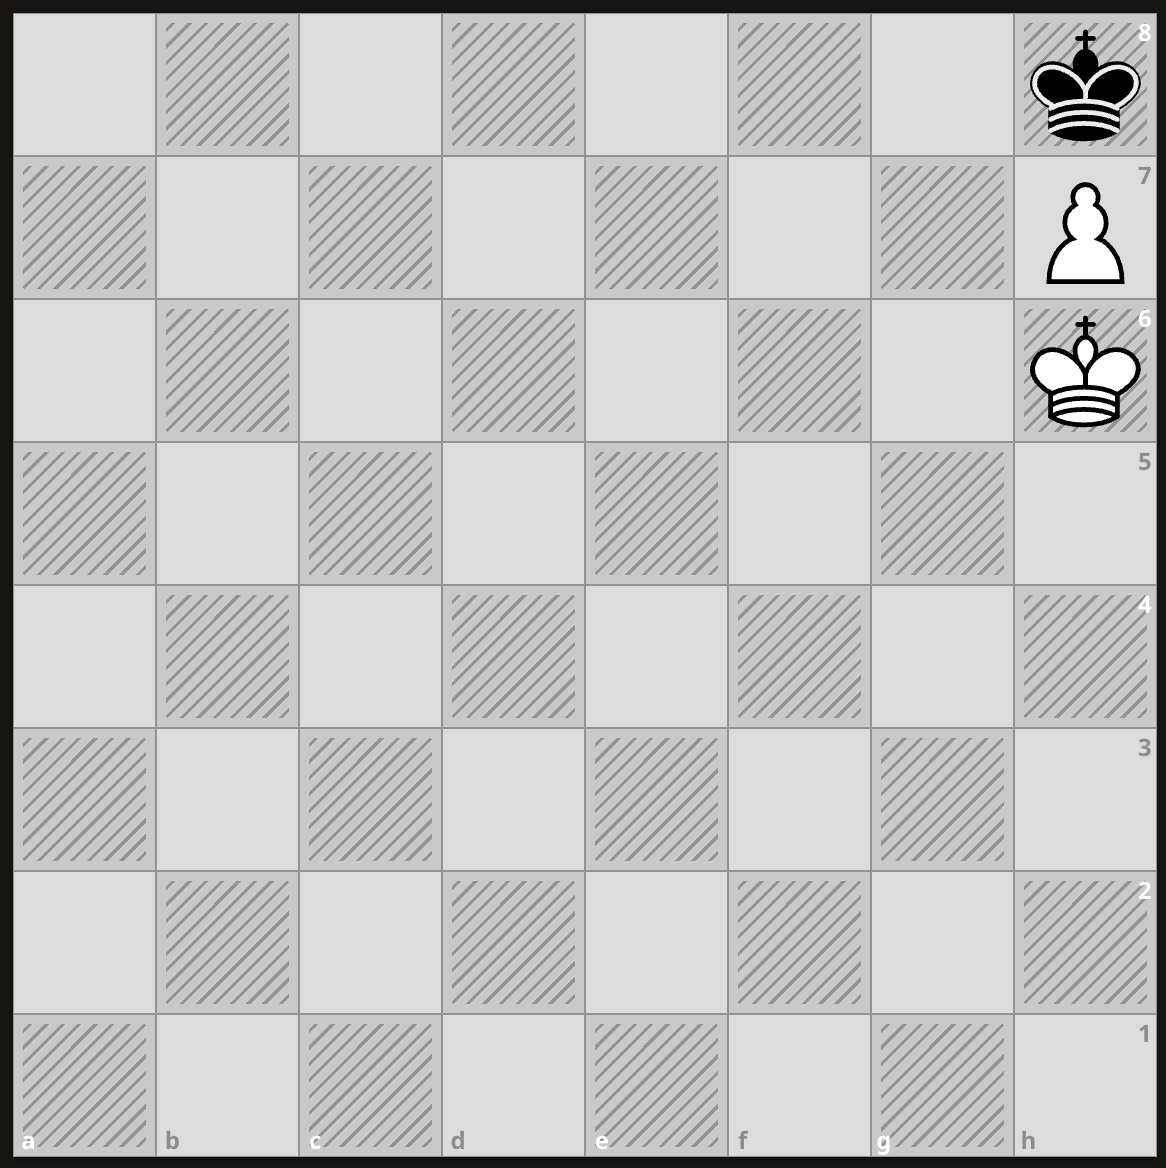
\includegraphics[width=8.0 cm,height=8.0 cm]{ahogado_1.png}

\end{center}
\medskip


Otro punto a rescatar son  la posibilidades de empate contenidas en el conjunto \emph{Vs(q)}, pues en el juego hay dos variantes de este (que excluyen a las cuestiones prácticas): la primera es un ahogado, que podemos definir como una posición en la cual no existe una jugada legal\footnote{Legal en este contexto quiere decir que es un cambio de posición que no viole ninguna regla del juego.} posible para continuar el juego, como se muestra en la figura \emph{a}. La otra consiste en una secuencia de más de 75 \cite[p. 42]{feda_manual_2021} movimientos sin que ocurra una captura de pieza. Esta segunda forma de empatar podría analizarse bajo el limite $\tau$ que propone Zermelo, pues para posiciones como, por ejemplo, en las que solo hay 2 reyes en el tablero, sería posible pasar por todos los estadios disponibles en el tablero y que nunca haya un jaque mate, por lo que dentro de todas las secuencias posibles, no existe una posición en la que alguno de los jugadores pierda después del movimiento $s$.

En la practica del juego existen 2 variantes de tablas adicionales que quedan dentro del teorema pero es pertinente diferenciarlas. Una de ellas consiste en la repetición de movimientos, que a su vez se divide en 2, una se conoce como \textit{jaque perpetuo} y es una posición en la que un jugador se dedica a dar jaque de manera repetida con la intención de finalizar la partida utilizando una regla que dicta que si se repite una misma posición en el tablero se puede reclamar el empate \cite[p.p. 41-42]{feda_manual_2021} la otra es una repetición de movimientos que se da porque de progresar el juego con alguna secuencia distinta a aquella en la que se vuelve a la misma posición, uno de los jugadores se condenaría a la derrota\footnote{Y si no se esta en una posición perdedora, no hay razones para propiciar una derrota propia.}.

La otra consiste en la insuficiencia de material, como ya se mencionó existen posiciones -como la de los dos reyes- en la que es imposible concebir una figura de mate. Para posiciones particulares es imposible conseguir finalizar el juego con una victoria dado que no existiría manera de generar un jaque mate, pero hay que hacer la distinción entre esta y la de los 75 movimientos, pues se puede dar que para ciertas figuras de jaque mate\footnote{Particularmente la de alfil y caballo.} la dificultad de ejecutarlas sea tan alta para algunos jugadores que 75 movimientos no son suficiente, aunque sea posible forzar la victoria para el jugador con las piezas de ventaja. 

El rescatar estas situaciones tiene como objetivo mostrar que aunque el teorema de Zermelo comprende de manera general cómo es que a partir de una posición un jugador \emph{no pierde} después del movimiento $s$, en la práctica surgen cuestiones como la repetición de movimientos que a pesar de ser descartadas por Zermelo, estas pueden atender a un fin que no necesariamente sea solo práctico, sino que puede incluso que la secuencia ganadora tenga repetición en virtud de garantizar que uno de los jugadores no pierde.

Otra de las cuestiones que pueden generar confusión\footnote{Tanto si se es aficionado al juego como si se profundiza en la resolución de problemas.} es la cota $\rho$ la cual representa una cantidad de movimientos algo más complicada de abordar en términos prácticos, pues ¿qué determina la cantidad mínima de movimientos? Por ejemplo, en la siguiente posición juegan blancas y ganan:
\medskip
\begin{center}
    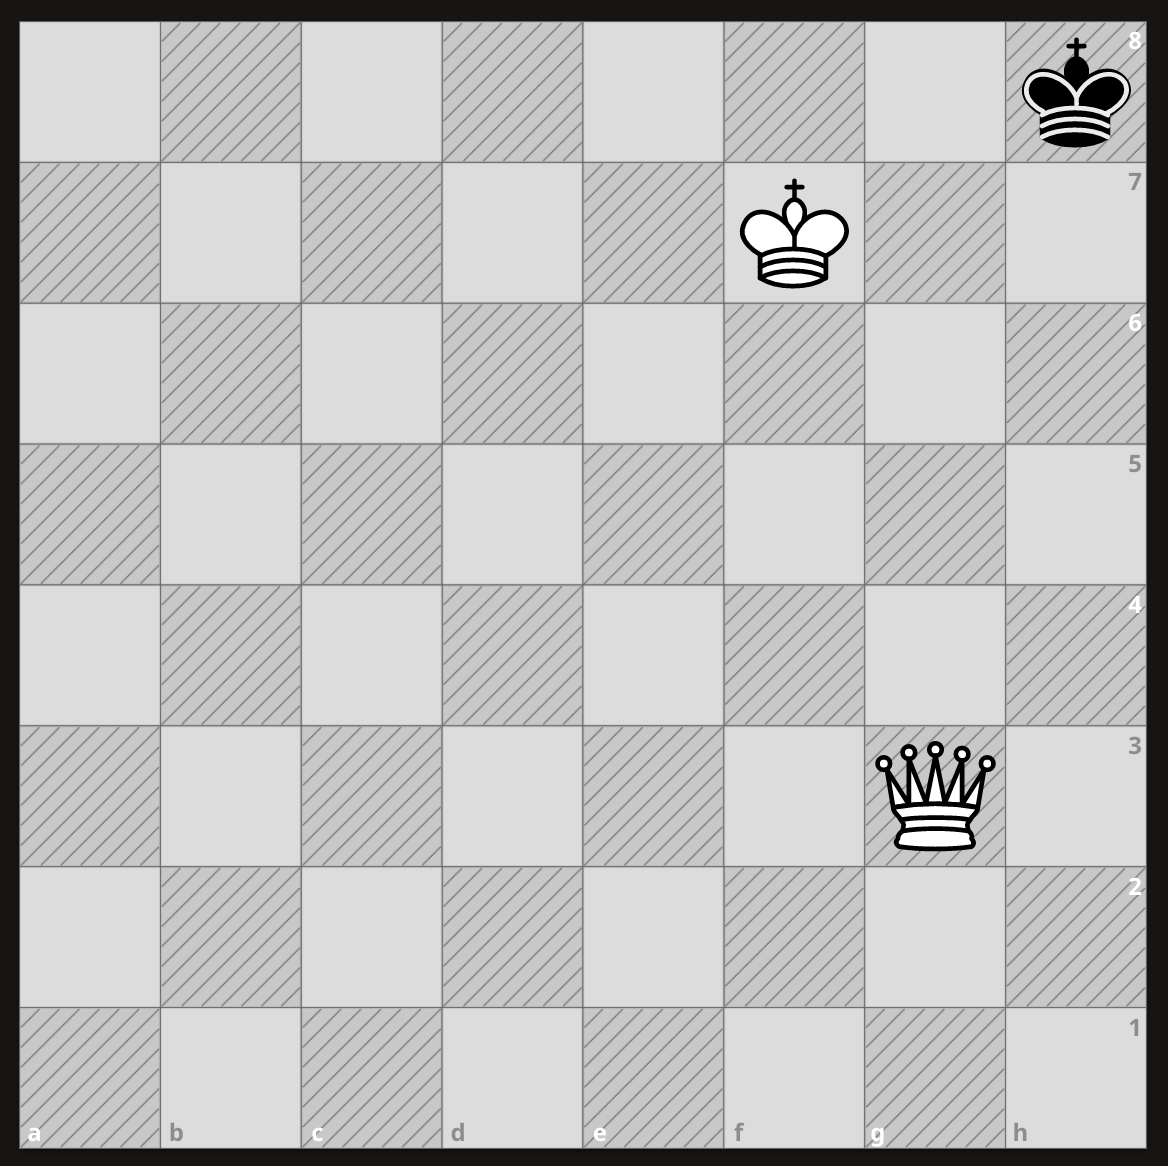
\includegraphics[width=8.0 cm,height=8.0 cm]{mate_en_1.png}
\end{center}

En términos prácticos lo mejor es conseguir la victoria del modo más rápido posible, tratar de alargar el juego parecería ser en virtud de cuestiones ajenas a este, pues si el objetivo es ganar ¿existiría una motivación que no sea ajena al juego para extender la duración de éste? Dicha cuestión se puede explorar más adelante, pero regresando al problema con $\rho$: en esta posición q juegan blancas y existen al menos 5 posiciones q distintas que finalizan el juego con una victoria para blancas en un solo movimiento, por lo que $\rho$ sería igual a 1, que es la cantidad mínima de movimientos necesarios para que blancas pueda forzar una victoria, pero existen muchas otras combinaciones de movimientos que son mayores a 1 y que aun así sostienen que blancas pueda forzar una victoria en a lo más $r$ movimientos, por lo que esta posición pertenece a \emph{Ur(q)} y es posible observar la cota $\rho$.

En contraste, véase la siguiente posición:
\medskip
\begin{center}
    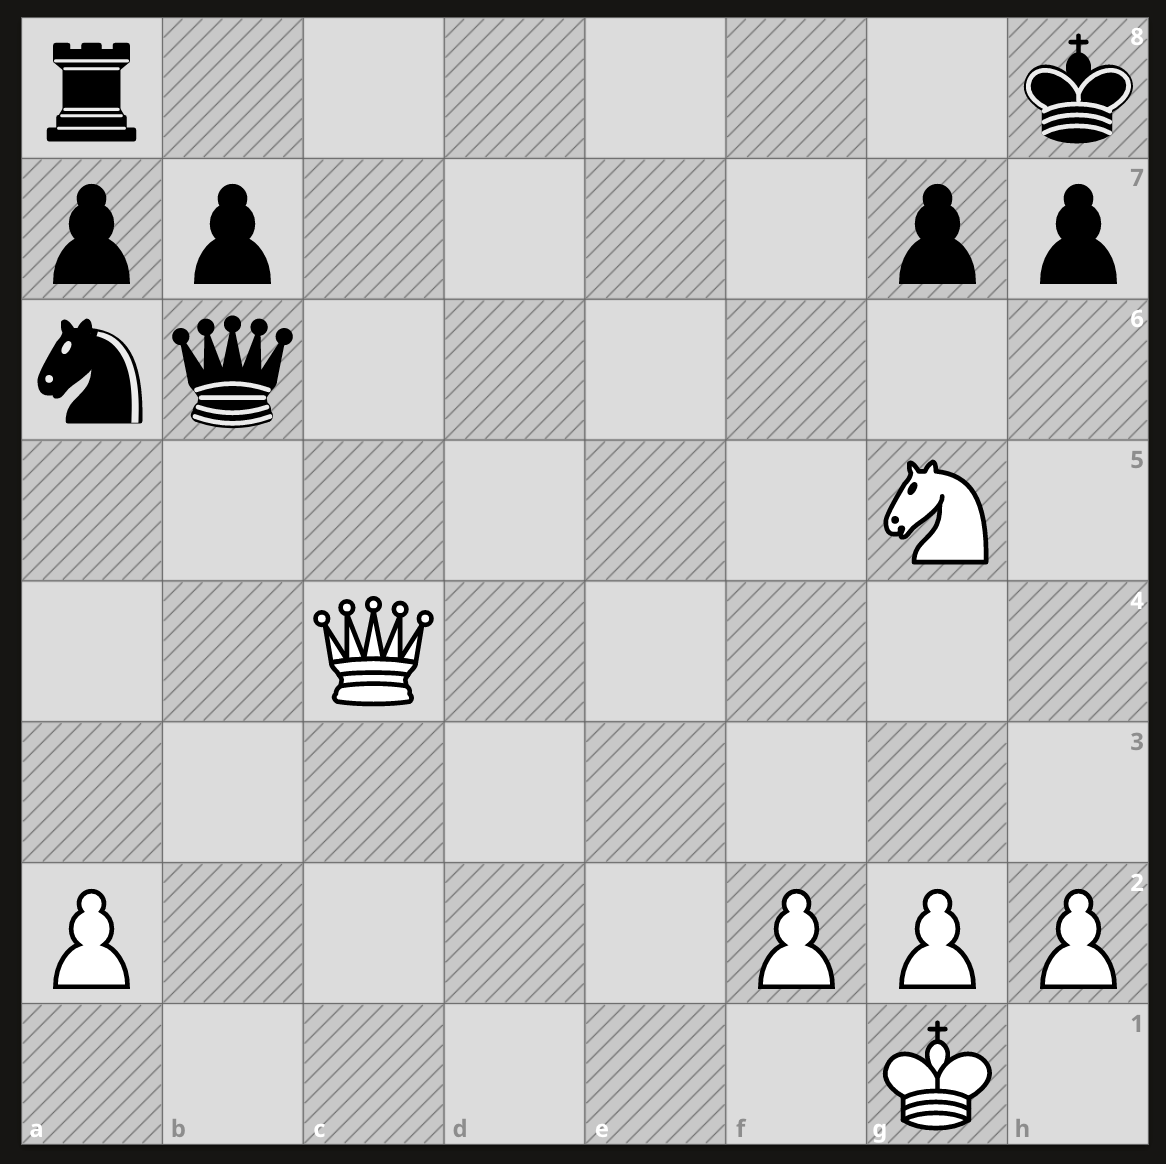
\includegraphics[width=8.0 cm,height=8.0 cm]{mate_de_la_coz.png}
\end{center}

En esta posición juega blancas y puede forzar una victoria en 4 movimientos, además, sin importar la respuesta de negras, blancas aún puede forzar una victoria, por lo que esta posición pertenece a $Ur(q)$, pero entonces ¿cuál es el problema? Pasa que blancas puede forzar la victoria en 4 movimientos, pero dependiendo de si negras se mueve a una posición $q$ o $q'$ es posible que blancas fuerce la victoria en solo 2 movimientos, por lo que ¿cuál sería el valor de $\rho$? ¿sería 2 o sería 4? Blancas va a ganar sin importar el camino que tome negras, pero dentro de todas las variantes en $Ur(q)$ sobre esta posición existe una en la que blancas gana en 2 movimientos, por lo que definir la cota inferior en la práctica parece un poco más complicado, ya que aquí se depende de que se considere como jugar de manera óptima.

Si jugar de manera óptima implica buscar la victoria en la cantidad mínima de movimientos y retrasar la derrota la cantidad máxima de movimientos posibles y ambos jugadores se enfrentan jugando con estas intenciones, la cota inferior $\rho$ debería ser 4, pues dadas las características particulares de la posición es el único camino en el que blancas puede forzar la victoria, sin embargo, si jugar de manera óptima implicara que, en caso y solo en caso de encontrarse en una posición perdedora, el jugador deba apresurar la derrota en la menor cantidad de movimientos, la cota $\rho$ debería ser 2. Esto depende totalmente de como se comporten los jugadores y cual sea la definición de jugar de modo óptimo.

Este tipo de preguntas parecen no tener lugar de manera clara dentro de la prueba de Zermelo, pero recordando que este teorema es un punto de partida para el desarrollo de la teoría de juegos es importante eventualmente establecer ciertas definiciones como el qué es jugar de el mejor modo posible (o de manera óptima), pero para efectos particulares de esta demostración, sirve como motivación para desarrollar la prueba dentro del caso particular del ajedrez y observar que a pesar de las contingencias y peculiaridades de los juegos para los que aplica el teorema, este se sigue cumpliendo a pesar de todo, pues no importa si los jugadores participan de manera óptima o si $\rho$ posee tal o cual valor, $\rho$ existe y puede acotarse al caso particular.

\section{Conclusiones}

\noindent El foco central del capítulo es la reconstrucción de la prueba. Darle otra estructura facilita la apreciación de -al menos- un par de problemas que quedan abiertos a la hora de enfrentarse a la aplicación del teorema en casos particulares. El ajedrez no es el único juego analizable, también lo son: el gato, las damas inglesas, las damas chinas o el Go. El comparar estos sistemas servirá para mostrar por qué el ajedrez es un caso que puede merecer un análisis más amplio, pues en el artículo original Zermelo arroja una conclusión muy interesante, pues menciona que de aplicarse al ajedrez, este perdería su carácter de juego \cite{zermelo1913anwendung}.

Esta afirmación por parte de Zermelo presenta una interrogante si se retrocede al principio de la prueba, pues afirma que de hecho ya se cuenta con un método para analizar posiciones y definir su resultado, como se hace en los \emph{problemas de ajedrez}. A pesar de que en el presente texto ya se expusieron un par de posiciones, dentro del mismo no se ofrecen herramientas para evaluarlas o escribir formalmente las secuencias, es por ello que la tarea del siguiente capítulo versa sobre ofrecer herramientas para representar las secuencias de posiciones y con ello desarrollar las consecuencias de intentar aplicar el teorema al ajedrez o en su defecto, analizar por qué podría no ser aplicable la estrategia ganadora, cuya existencia está garantizada por el teorema.

\chapter{Aplicación del teorema de Zermelo y los \textit{problemas de ajedrez}}
\markboth{CAPÍTULO 2}{Problemas de Ajedrez y el teorema de Zermelo} % encabezado 
\section{Introducción}

\noindent El siguiente capítulo posee la intenci\'on de exponer el proceso de aplicaci\'on del teorema de Zermelo a diferentes sistemas regidos por \'el, como lo son --para este caso particular-- el juego de gato, las damas inglesas y eventualmente el ajedrez. Es importante justificar por qu\'e se invertir\'a tiempo en estudiar sistemas banales como el gato o meramente l\'udicos como las damas antes de dar el paso al ajedrez, pues se pretende exponer cómo es que a medida que se vuelven m\'as elaborados los sistemas tambi\'en se vuelve muy superior la complejidad de encontrar la estrategia que los resuelve.

Para el caso del gato aunque parece que hay demasiadas variantes, el juego constante lleva a los humanos a desarrollar casi por intuici\'on la estrategia con la que pueden nunca perder, mientras que para el caso de las damas, aunque esta estrategia existe y ha sido encontrada, el implementarla para los humanos parece imposible, pues la cantidad de posiciones es tan alta que simplemente no parece factible que un ser humano pueda retenerlas, procesarlas y preservar el algoritmo que lo lleva al resultado del juego --que al igual que en el gato, es un empate--.

Comparar estos sistemas permite hacer un an\'alisis un poco m\'as extenso sobre el caso del ajedrez, pues por el teorema de Zermelo se sabe que existe una estrategia ganadora, pero ¿es posible encontrarla?, ¿ya se ha encontrado?, ¿es implementable? El proceso de resolución de problemas sumado con la práctica y estudio de finales muestra que se puede encontrar la estrategia que fuerza un resultado particular, en cuyo caso ¿qué ha impedido que ésta sea descubierta?

\section{Aplicación del teorema}

\noindent El teorema de Zermelo puede ser evidenciado a trav\'es de diferentes sistemas para corroborar que si es el caso que cumplen las condiciones, entonces existe una estrategia que fuerza el resultado al que el juego est\'a determinado. Si bien esto puede parecer trivial por la prueba que realiz\'o Zermelo, encontrar la estrategia exacta dista de ser trivial, pues es una herramienta que podr\'ia banalizar algunos juegos o sistemas, como pasa con el gato, juego en el que algunos infantes y adolescentes se pueden entretener, pero en cuanto se topan con el hecho de que si juegan de manera ideal siempre ser\'a un empate, le pierden todo inter\'es. 

El proceso de aplicaci\'on parece crecer de manera distinta en cada juego. Aunque sistemas como el gato parezcan sencillos, crecen de manera considerable, mientras que sistemas como el de las damas inglesas --conservando una cantidad sencilla de reglas-- crecen de manera monstruosa. Este proceso arroja resultados pr\'acticos del teorema de Zermelo para diversos sistemas. Para todos los sistemas regidos por el teorema existe una secuencia ganadora y es posible encontrarla de manera inductiva. Pero que sea posible encontrarla no quiere decir que los seres humanos o sus creaciones tengan la capacidad de hacerlo. 

La exposición de los siguientes casos mostrará cómo se puede pasar de resolver un juego en unos d\'ias a tardar 15 años o más en encontrar la secuencia \'optima. Además se dará un acercamiento al ajedrez desde los problemas para observar que, en efecto, se puede calcular el resultado determinado para una posición, pero que el proceso de deducción --si se hace sin alguna heurística que lo restrinja-- puede crecer en pocos pasos haciendo una progresión superior a exponencial.


\subsection{El caso del juego de gato}

\noindent Si se repite el proceso realizado para los posibles estadios de ajedrez con el juego de \emph{gato}\footnote{También conocido como \emph{3 en línea} o \emph{Tic tac toe}.}, es posible exhibir de manera casi inmediata qué tanto crece el juego. Esto es relevante ya que este sistema cuenta con las caracter\'isticas necesarias para que sea regido por el teorema --por lo que sería comparable al ajedrez--. Posee informaci\'on completa, suma Zero, es de dos participantes y tiene excenci\'on de suerte.

Véase del siguiente modo: el juego de gato tiene un tablero de 9 casillas, en cada casilla solo puede haber uno de dos símbolos, una $\times$ o un $\circ$. Los movimientos son necesariamente alternados, a cada jugador le corresponde solo uno de los símbolos y gana el primer jugador en alinear 3 de sus símbolos en horizontal, vertical o diagonal dentro de las 9 casillas del tablero. A partir de ello, es posible modelar el juego entero utilizando combinatoria.

La primera jugada tiene 9 espacios del tablero disponibles, la segunda 8, la tercera 7 y as\'i sucesivamente, es decir $9!$ con ello tenemos todas las posibles partidas si inicia un jugador, as\'i que solo habr\'ia que doblar este numero para tener todas las posibles partidas de gato, por lo que parecería que la formula sería $9!\cdot(2)$. Si se añade una regla que indique qué símbolo debe utilizar el jugador que haga el primer movimiento, incluso se podría descartar la necesidad de doblar las permutaciones del tablero, pues en aquellas en las que haya un numero impar de casillas ocupadas corresponden al turno del jugador que no empezó el juego y por el contrario, si la posición tiene un número par de casillas ocupadas, será turno del jugador que empezó el juego.

Por ello, se tiene una cantidad de 362880 partidas posibles de gato. Como este juego se encuentra regido por el teorema --dadas las características mencionadas previamente-- se sabe entonces que está determinado y que existe una estrategia \'optima. Como de hecho se puede evaluar una posición de manera similar a como se hace con los problemas de ajedrez, se podría evaluar la posición anterior, y la anterior y así sucesivamente hasta llegar al punto de partida. Además se sabe que la longitud de una partida es de a lo más 9 movimientos, por lo que evaluar de manera retro-inductiva cada posición entregaría secuencias de a lo más 9 pasos.

Este proceso por fuerza bruta resultaría poco práctico para los humanos, pero para los ordenadores no sería tan complicado de resolver. Es por ello que los seres humanos pueden centrarse en desarrollar una heurística que reduzca la necesidad de calcular tantas posiciones, como por ejemplo, buscar equivalencias en el tablero. Considérese por ejemplo las siguientes dos posiciones: 

\begin{center}
    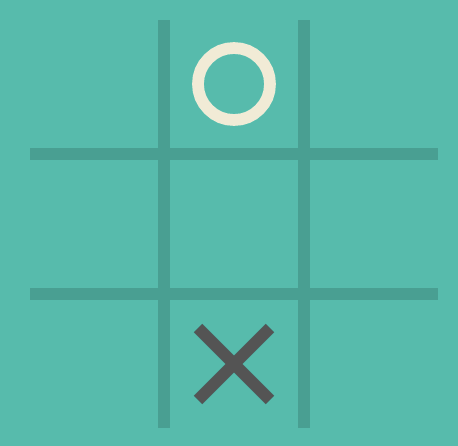
\includegraphics[width=5.0 cm,height=5.0 cm]{gato1.png} \hspace{20pt}
    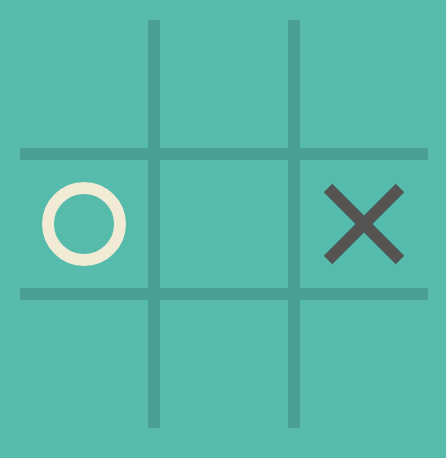
\includegraphics[width=5.0 cm,height=5.0 cm]{gato2.png}
\end{center}

Ambas posiciones son diferentes, pero ¿qué pasa si se consideran desde distintas perspectivas? Si se considera que los dos jugadores están viendo el tablero desde la misma posici\'on, ambas posiciones se consideran distintas, pero si en la segunda posición, los jugadores vieran el tablero con el símbolo $\times$ frente a ellos, entonces parecería que ambas posiciones son iguales:

\begin{center}
    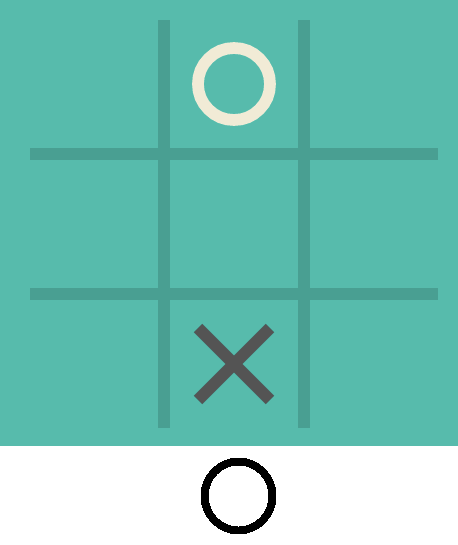
\includegraphics[width=5.0 cm,height=6.0 cm]{gato1.1.png} \hspace{20pt}
    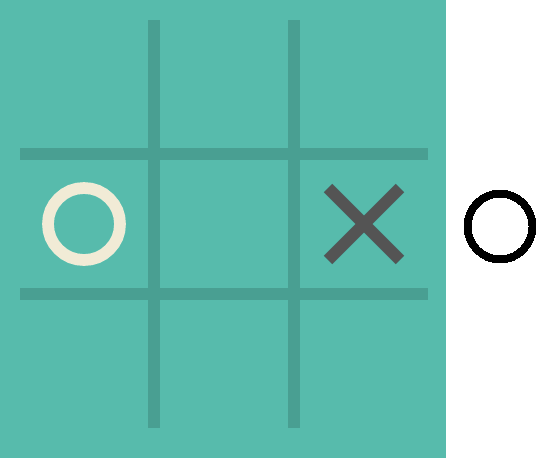
\includegraphics[width=6.0 cm,height=5.0 cm]{gato2.1.png}
\end{center}

De ser así, parecería que entonces existen posiciones equivalentes, por lo que existiría el caso en que 2 o más partidas sean iguales si se les observa desde una perspectiva distinta. Hay que añadir una situación adicional, pues hay posiciones cuya equivalencia parecería no ser evidente simplemente cambiando la posición desde la que se observa el tablero, por lo que se tendría que considerar una perspectiva en \emph{espejo} como la siguiente:

\begin{center}
    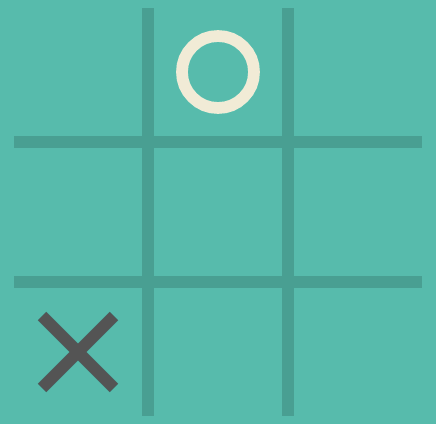
\includegraphics[width=5.0 cm,height=5.0 cm]{gato3.png}\hspace{20pt}
    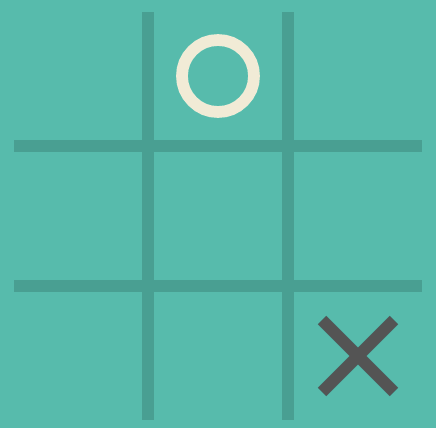
\includegraphics[width=5.0 cm,height=5.0 cm]{gato4.png}
\end{center}

Con este tipo de estrategia parecería que hay 3 puntos del tablero particularmente relevantes: el centro, la esquina y centro-orilla, pero ¿cuál es el propósito de rescatar estas 3 casillas? Sucede que cualquier movimiento inicial puede ser representado por estos cambios de perspectiva y sólo serían necesarios dos movimientos para saber que tipo de perspectiva aplicar, por lo que si se evalúan todas las partidas que surgen a partir de las siguientes 3 casillas:

\begin{center}
    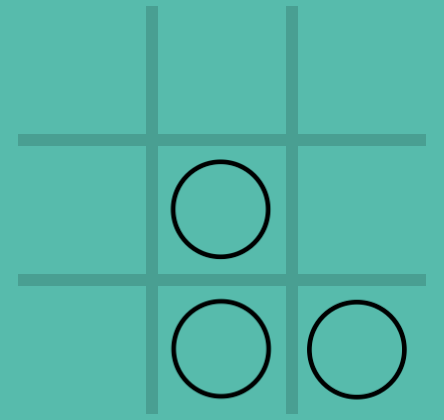
\includegraphics[width=5.0 cm,height=5.0 cm]{gato5.png}
\end{center}

Se tendría la evaluación para todas las partidas posibles, por lo que en lugar de $9!$ la formula sería $3 \cdot 8!$ donde 3 representa los 3 posibles inicios relevantes --esquina, centro y centro-orilla-- y el $8!$ sigue el razonamiento anteriormente utilizado para la operación factorial.

Para este punto se han reducido demasiado las posibles partidas a calcular y puede continuar el proceso, pues todas estas partidas son de 9 movimientos. Como la cantidad mínima de movimientos necesarios para que alguien gane es de 5 se podrían descartar las partidas que continúan a pesar de que ya haya un ganador en el tablero. Así la cantidad de partidas a evaluar se vuelve cada vez menor por lo que eventualmente se llega a que el juego de gato está determinado a un empate, si ambos jugadores se desempeñan de manera óptima, ninguno de los 2 perderá. Con ello se observa que se cumple el teorema de Zermelo, pues en un sistema de características particulares existe una estrategia que garantiza un resultado determinado considerando que ambos jugadores se desempeñen del mejor modo posible. 

Esta generalización muestra que es posible encontrar dicha estrategia por fuerza bruta y que se puede desarrollar una heurística para volver eficiente el cálculo para humanos --y probablemente también sea implementable en ordenadores--. Una respuesta a cu\'al ser\'ia la estrategia ganadora particular se puede construir implementando el proceso desarrollado en \emph{A Fractal Guide to Tic Tac Toe} \cite{stewart2000fractal} que consiste en construir semi-fractales a partir de las variaciones de las posibles posiciones iniciales del juego. Se dice que son semi-fractales ya que la cantidad de posiciones es finita, por lo que no se seguir\'ia reproduciendo el patrón de manera indefinida, como sí pasa en los fractales. Esta estructura se ve del siguiente modo:

\begin{center}
    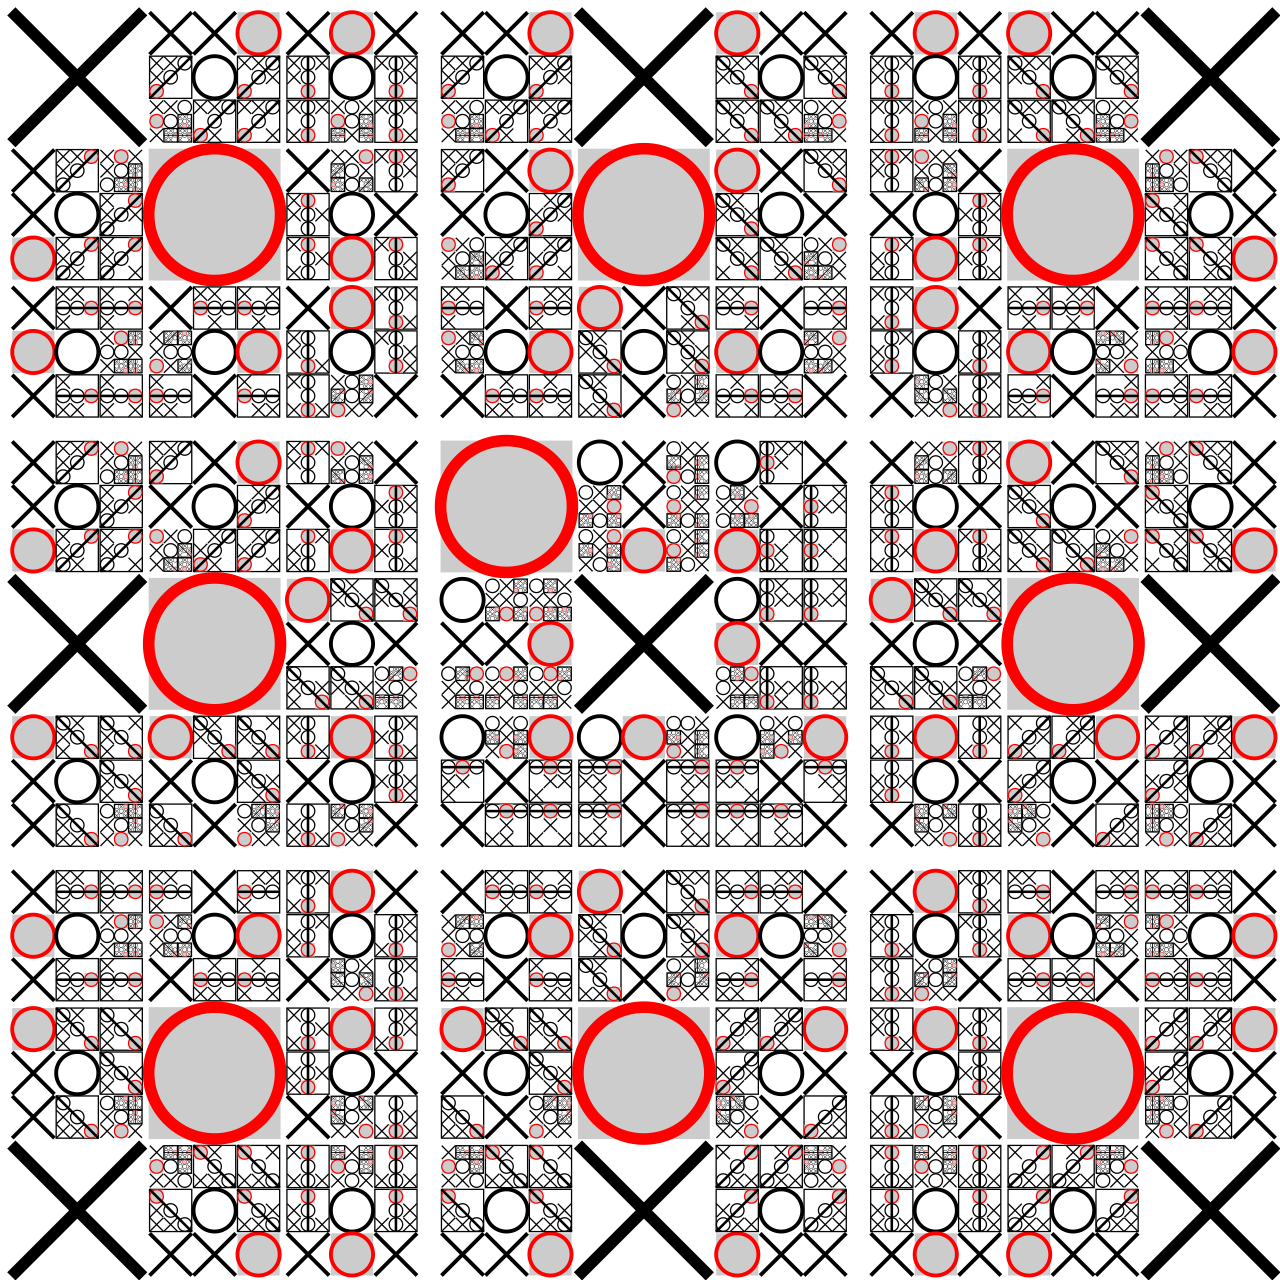
\includegraphics[width=10.0 cm,height=10.0 cm]{Tictactoe-O.svg.png}\footnote{El modelo representa las secuencias en las que $\circ$ juega iniciando en el centro, posici\'on en la cual puede forzar unas tablas si es que $\times$ se equivoca y un empate si ambos juegan del mejor modo posible.}
\end{center}

De ella es posible inferir las secuencias ganadoras para el modelo que propone a 9! como la totalidad de partidas posibles, de hecho podr\'ia ser restringido al propuesto de considerar algunos inicios particulares y tomar el resto de partidas como equivalentes, pero eso resultar\'ia menos vistoso desde la perspectiva de los fractales. Es as\'i como puede observarse entonces, tanto que el juego es finito, como una búsqueda de las estrategias ganadoras --que conducen al empate--. 

\subsection{El caso de las damas inglesas}

\noindent Las damas, por otra parte, son un juego considerablemente m\'as complejo\footnote{Hay que añadir que la complejidad tiene varias dimensiones, no solo el aumento de posibles posiciones o partidas.} que el gato. Para este se considera un tablero idéntico al del ajedrez, que consta de 64 casillas dadas por 8 filas y 8 columnas, adem\'as de s\'olo 24 piezas, 12 para blancas y 12 para negras. Tambi\'en consid\'erese que a pesar de que el tablero contiene 64 casillas, el juego en realidad se desarrolla en la mitad dado el movimiento de las piezas, que en el caso de las damas inglesas es s\'olo en diagonal.

Este juego tiene un par de facilidades de evaluaci\'on respecto al ajedrez. Por ejemplo: en el ajedrez es posible que un caballo se mueva y regrese a su posic\'on de inicio, en teor\'ia podr\'ia incluso pasar por todas las casillas libres del tablero antes de poder regresar a su estado inicial, secuencia que ser\'ia totalmente legal y contenida en la totalidad de partidas posibles\footnote{De hecho, podr\'ia reptirse hasta tres veces en diferente orden y segur\'ia siendo legal, por lo que para el termino de esa secuencia se regresar\'ia a la posici\'on original.}, mientras que en las damas a menos que se \emph{corone}, ninguna de las piezas tiene la posibilidad de retroceder a una posici\'on anterior. Esto aunado a que en ciertas variantes del juego\footnote{Sucede que las reglas llegan a variar de acuerdo a la localidad en la que uno se encuentre.} hay movimientos que son obligatorios --como capturar una pieza-- el proceso de calcular las posibles ramas a partir de una posici\'on dada es mucho m\'as sencillo y con menos posibles secuencias\footnote{Aunque el juego crece de manera exponencial.}.

Las damas ya han sido matem\'aticamente resueltas. En 2007 se public\'o el trabajo de Jonathan Schaeffer \cite{schaeffer2007checkers} en el que despu\'es de encontrar que el juego tiene $5\times10^{20,000}$ posibles posiciones y un arduo trabajo de c\'aculo, mostr\'o que las damas est\'an determinadas a un empate \cite[p. 1518]{schaeffer2007checkers}. La principal motivaci\'on para realizar este trabajo surge de alimentar el motor Chinook desarrollado para jugar damas contra los jugadores m\'as fuertes del mundo. En 1990 Chinook obtuvo el derecho para jugar contra el campe\'on mundial de damas, Marion Tinsley, quien por poco logra vencer a Chinook. Con esto se mostraba que Chinook era muy superior a los jugadores humanos, brecha que solo incrementaba con la evoluci\'on de la tecnolog\'ia.

Este trabajo se public\'o en \emph{Checkers is solved}, art\'iculo en el cual, adem\'as de narrar una breve introducci\'on hist\'orica al problema, se presenta c\'omo es que se empez\'o a afrontar el problema de resolver el juego de damas. El motor se sirve de 3 herramientas principales para resolverlo. En primer lugar, una base de datos que consta de finales, lo que permite hacer una búsqueda retro-inductiva\footnote{La retro-inducci\'on empieza su an\'alisis desde un estadio particular del tablero para obtener las posiciones previas, en lugar de tomar una inicial y generar las subsecuentes.} para encontrar secuencias ya determinadas. En segundo, un gestor de arboles de prueba, que permite decidir y limitar que posiciones deben ser exploradas. En tercero una herramienta que resuelve la posici\'on que entrega el gestor de \'arboles. Esta herramienta consta de otro par de componentes auxiliares que eval\'uan la posici\'on par apoder entregar un resultado que sea \'util para la pr\'actica \cite[p. 1519]{schaeffer2007checkers}, idealmente decidir si la posici\'on es la mejor linea que se pueda jugar\footnote{La mejor linea ser\'ia aquella en la que ninguno de los jugadores cometa un error.}.

Este es un primer paso en acercarse al proceso de resoluci\'on de problemas en el ajedrez. En el caso de las damas no solo se pueden analizar las posiciones que surgen a partir de una inicial, sino que tambi\'en es posible tratar de ubicar de qué posiciones surge una en particular. Esto resulta m\'as \'util que en el gato y m\'as sencillo que en el ajedrez, pues a partir de una posici\'on ganadora se puede retroceder para ubicar al menos un par de posiciones anteriores que conducen al mismo resultado. Esta situaci\'on permite minimizar la cantidad de posiciones a calcular por inducci\'on, pues en lugar de calcular dos ramas que lleven al mismo resultado, se puede deducir con anterioridad que de encontrarse en alguna de esas posiciones, el resultado est\'a determinado.

En contraste con el juego de gato, las damas son un juego mucho m\'as complicado de resolver. Se considera que las damas, aunque están resueltas, lo están hecho de manera \emph{d\'ebil} \cite[p. 1518]{schaeffer2007checkers}. Esto quiere decir que a pesar de que se conoce el resultado y la estrategia \'optima, no se conoce para todas las secuencias posibles, pues las herramientas diseñadas para evaluar el juego descartan posiciones que parecer\'ian indicar una gran desventaja para uno de los jugadores, sin presentar necesariamente la secuencia que finaliza con una victoria. 

Mientras que el juego de gato parece que se puede resolver con creatividad y c\'alculo en un corto lapso del tiempo, hacer lo mismo para las damas tom\'o alrededor de 15 años, e incluso eso no garantiza una resoluci\'on \emph{fuerte} del juego. La diferencia de tiempo es abismal, pero las herramientas que surgen a partir de estos dos resultados son valiosas para enfrentarse a otros sistemas. La inducci\'on, la retroinducci\'on y descartar las variables que parecieran dejar en clara ventaja a un jugador son efectivas para evaluar juegos distintos, particularmente el ajedrez. A pesar de esto, hay que considerar que el que sea evaluable o computable, no quiere decir que los seres humanos o sus creaciones sean capaces de hacerlo. En esa situaci\'on, ¿de qu\'e manera hay que afrontar los problemas de ajedrez y el juego en s\'i?

\section{Una base para resolver problemas de ajedrez}

\noindent La resolución de problemas requiere de 2 herramientas indispensables: la notación y una heurística para escoger la mejor secuencia de posiciones. La primera se justifica en el hecho de poder describir, compartir y almacenar las secuencias a ciertas posiciones, ya sea con el fin de estudiarlas, preservarlas, mostrárselas a un tercero o simplemente exhibirlas. Además es conveniente conocer cuál es el consenso --o al menos bajo qué criterios generales-- se resuelven los problemas de ajedrez.

Llegar a dar una respuesta última parecería complicado, pues hacer una evaluación finales como de rey y torre contra rey dista de aquella que se haría a una posición de apertura o medio juego, e incluso frente a otro tipo de finales, al menos en el caso de cómo los humanos evaluamos los problemas. El proceso realizado para el caso del gato y de las damas también es aplicable al ajedrez, de hecho parecería que es el proceso descrito por el teorema de Zermelo, pero la práctica del juego muestra que hay diferencias sustanciales en cómo los humanos juegan al ajedrez. Por ahora, solo se dará una perspectiva general de cómo es que se resuelven los problemas y eventualmente se observará qué pasa cuando se aplica el teorema.

\subsection{La notación}
\noindent Es posible presentar una forma de seguir las secuencias de manera simple a partir de una posición dada utilizando dos elementos: conocer la posición sobre la cuál partirá el análisis y la notación algebraica, desarrollada para escribir secuencias de movimientos a partir de la posición inicial y que además funciona para cualquier posición legal concebible. Este sistema algebraico surge a partir de la evolución del sistema descriptivo, que, a pesar de ser útil, resultaba poco práctico por lo extenso que llegaba a ser decir una jugada, junto con otros factores.

%%\footnote{La notaci\'on algebraica es la \'unica utilizada en las competencias de la FIDE desde 1997 } recordar meter nota sobre la fecha

Entender el sistema algebraico no es complicado, lo primero a tener en cuenta es que dependiendo del idioma habrá una variación respecto a la notación. Para el español se usan las letras T, C, A, D y R para representar a la torre, el caballo, el alfil, la dama y el rey respectivamente\footnote{Para el inglés se usan las letras R, N, B, Q y K respectivamente. Es útil conocer esto ya que ésta es de las notaciones más comunes.}. Los peones tienen una particularidad, pues estos no se señalan con alguna letra; para marcar los movimientos que realizan únicamente se indica cuál es la casilla de llegada del peón, mientras que para el resto de movimientos también se señala que pieza se ha movido y cuál es la casilla de llegada. Salvo un par de excepciones\footnote{Por ejemplo, cuando dos piezas del mismo tipo pueden llegar a la casilla que se indica; de ser así se indica la columna en la que se encuentra la pieza a mover. Si ambas están en la misma columna, en su lugar se indica la fila.}, únicamente se indica la casilla de llegada y si en ese movimiento hay alguna otra situación particular que señalar, tales como: la captura una pieza, si ocurre un jaque, si ocurre un jaque mate, entre otras.

Para describir las casillas se utiliza una notación de pares ordenados en la que se indica la columna y la fila en la que se encuentra la casilla. A cada fila se le designa un número del 1 al 8 siguiendo el orden natural de este conjunto de números. A cada columna se le designa una letra desde la A hasta la H siguiendo el orden alfabético de las letras. Al ser pares ordenados cada casilla cuenta con una letra y un número para identificarla y por convención primero se indica a que columna pertenece y luego a que fila; por ejemplo, la casilla inicial del rey blanco sería \emph{e1}, la de la dama blanca sería \emph{d1}, etc. De igual modo por convención, aunque dentro del tablero las columnas suelen marcarse con letras mayúsculas, en la notación se señalan con letras minúsculas, ya que las letras mayúsculas están reservadas para las piezas \cite[p. 53]{feda_manual_2021}.

Los símbolos adicionales con los que se cuenta --estrictamente para describir los movimientos-- son: un signo de suma $+$ para señalar que el movimiento realizado pone en jaque al rey oponente, un $\#$ para marcar que el movimiento ha conseguido dar un jaque mate, aunque también es posible marcarlo con dos signos de suma $++$, un  $o-o$ para marcar un enroque corto, un $o-o-o$ para marcar un enroque largo, una $\times$ para marcar que se ha capturado a la pieza que se encontraba en la casilla de llegada, y un signo de igual $=$ para cuando se corona un peón indicar cuál es la pieza que le sustituye. Adicional a esto es posible encontrar en muchas revistas, módulos de análisis, libros y prácticamente en todo texto y herramienta relativa al juego el uso de los símbolos “?” y “!”, donde el primero indica que la jugada realizada es una imprecisión o error, y el segundo denota una jugada particularmente buena y poco intuitiva, pero dado que estos símbolos son propios de análisis posteriores a la partida se quedarán en esta mención.

Como ya se dijo, con la notación algebraica sólo se menciona la casilla de llegada de las piezas, esto no representa problemas para la posición inicial, ya que en el ajedrez clásico esta es única, por lo que partiendo de esto es posible describir toda una partida solo con la notación. Un movimiento se ve de la siguiente manera: 

  \Large\[D\times d4+\]
    
\normalsize
Donde $D$ indica la pieza que se mueve y es el primer elemento para anotar en cada movimiento; como ya se mencionó, el peón tiene una situación particular, pues no se indica una letra para él, pero en caso de que en su movimiento realice la captura de una pieza se indica antes del signo $\times$ la columna en la que se encontraba el peón antes del movimiento\footnote{Por ejemplo, si un peón de la columna d captura una pieza en e4, se escribiría $d\times e4$.}. $\times$ indica que se ha capturado una pieza en este movimiento y va después de la letra que simboliza la pieza que se ha movido y antes de la casilla de llegada, $d4$ indica la coordenada de la casilla a la que se ha movido la pieza del jugador en turno y $+$ indica que en ese movimiento se ha dado un jaque al rey oponente, puede también ser el símbolo de jaque mate en cualquiera de sus variantes, ya sea $++$ ó $\#$ y este siempre va después de la casilla de llegada.

Esto es solo un panorama general de cómo es que se lee la notación y cómo se interpreta, ya que aclarar todas las situaciones posibles convertiría este texto en una suerte de manual incompleto de cómo se juega al ajedrez, así que para cualquier contingencia que no quede señalada de manera precisa de acuerdo a las necesidades del texto y al ajedrez en particular es posible consultar el manual oficial de la FIDE (Fédération Internationale des Échecs) o de la FEDA (Federación Española de Ajedrez), en donde se encuentran: las reglas básicas del juego, la notación, el objetivo del juego y sus reglas particulares, hasta regulaciones acerca de éste como competencia, entre otras cosas.

\subsection{El proceso de resolución}

\noindent El proceso que suelen seguir los seres humanos a la hora de resolver problemas consta del cálculo de variantes y el seguimiento de estrategias que lo restringen. Muchas de estas estrategias parecen difíciles de explicar, pues son obtenidas por la práctica y el estudio constante del juego. Por ahora no se ahondará mucho en los fenómenos de análisis más elaborados o ambiguos --como el golpe de vista-- y el proceso que se explica a continuación se servirá de alternativas que parecen más evidentes de utilizar para cualquier persona.

El cálculo dentro del ajedrez --generalmente-- consiste en la consideración de un árbol de variantes  a partir de una posición, es decir, considerar las posibles posiciones que surgen a partir de seguir las reglas particulares del juego para encontrar una estrategia que fuerce el mejor resultado para el jugador. Este proceso parecería ineficiente ya que en el ajedrez las variantes crecen de manera exponencial\footnote{E incluso superior a la exponencial}, por ello resulta necesario empezar a implementar ciertas estrategias para poder reducir la cantidad de líneas de juego a analizar para resolver los problemas y enfrentarse a cualquier posición. Una alternativa que parecería eficaz sin recurrir a métodos de juego más elaborados y específicos sería empezar por restringir las posibilidades de movimiento del oponente, con la intención de analizar primero las secuencias que son necesariamente más cortas que el resto. Con esto presente ¿cómo se resolvería la siguiente posición?


\medskip
\begin{center}
    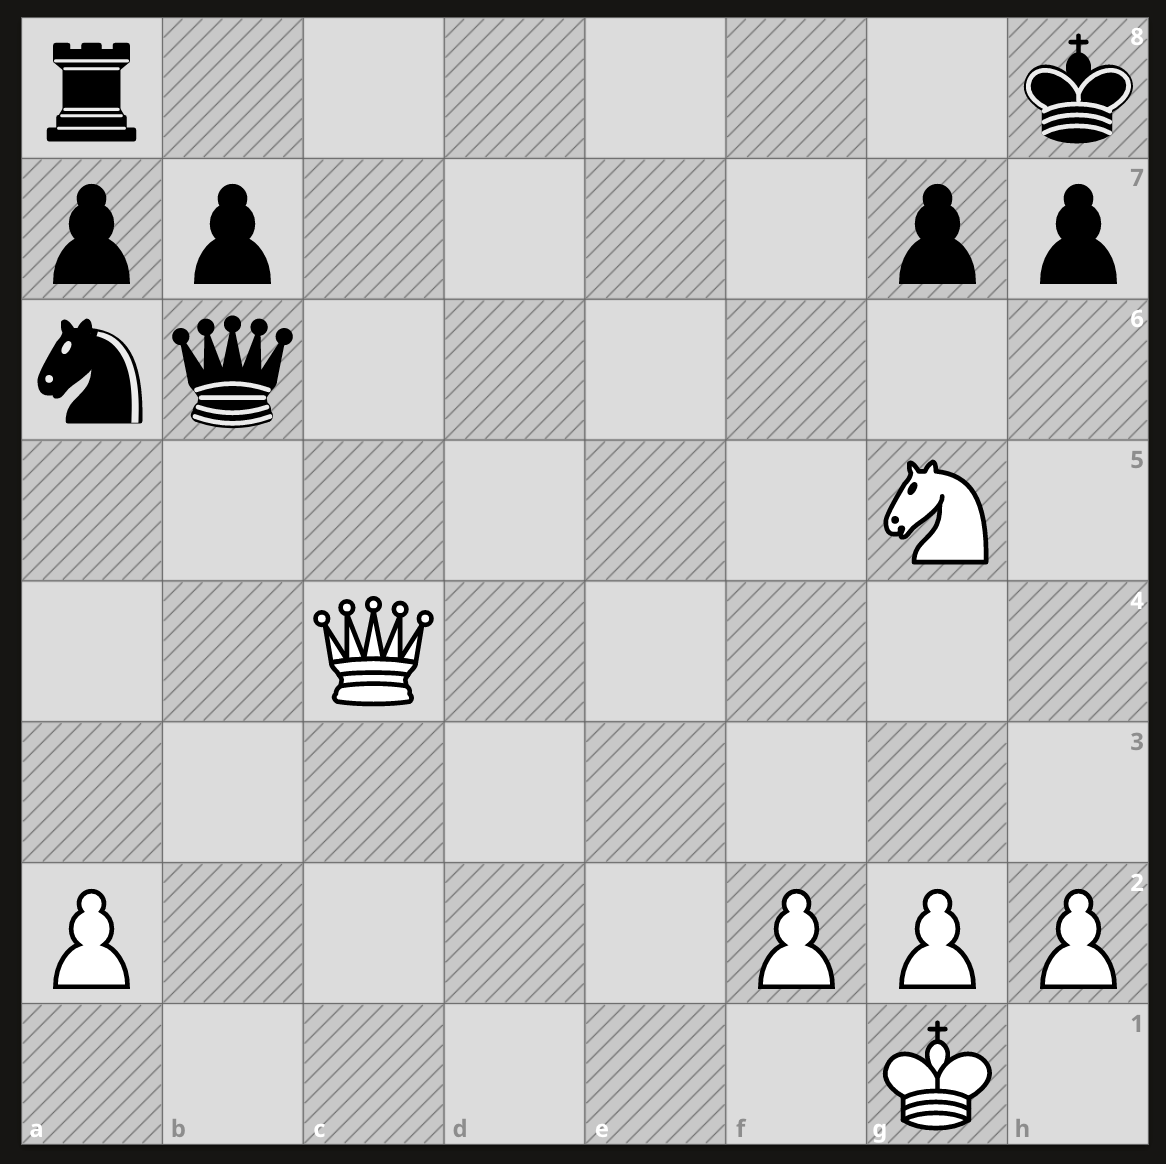
\includegraphics[width=8.0 cm,height=8.0 cm]{mate_de_la_coz.png}

    Juegan blancas, mate en 4.
\end{center}

Siguiendo las pautas anteriores, se puede razonar del siguiete modo: existen 3 jugadas que limitan las posibilidades de las piezas negras a dos movimientos o menos, estas serían 1. Dc8+, 1. Dg8+ y 1. Cf7+; si se opta por la primera entonces las piezas negras pueden responder tanto con 1.  …  Txc8 como con 1. … Dd8, si se opta por 1. …. Txc8 el jugador con blancas puede continuar con la idea de restringir posibilidades jugando 2. Cf7+, la única respuesta disponible sería. 2. ….  Rg8, a lo cual la única jugada siguiente que restringe sería 3. Ch6+, y después de 3. …   Rf8 no existe una jugada que limite las posibilidades del negro, pero dado que ya han pasado 3 movimientos el siguiente debería ser un mate para que se cumplan las especificaciones del problema, pero negras cuenta con la jugada 4. … Db1+, entonces si negras juega con 1. …  Txc8, blancas se encontraría eventualmente en una desventaja de material\footnote{La desventaja material es una situación en la que un jugador tiene menos piezas que el rival.}, por lo que analizar la variante con 1. …  Dd8 sería infructífero para negras pues en esa posición negras tiene la ventaja no jugándola, además de que esta detona una cantidad muy superior de variantes a calcular, entonces incluso si con esa jugada negras vuelve a encontrarse en una ventaja material, lo conveniente es hacerlo en la menor cantidad de movimientos posible.

Si se opta entonces por 1. Dg8+ negras tiene dos movimientos, ya sea 1. … Txg8 o 1. … Rxg8, si negras opta por 1. … Txg8 entonces blancas puede dar un mate con 2. Cf7, por lo que ese movimiento no conviene a negras, y si opta por 1. … Rxg8 blancas no puede limitar los movimientos disponibles con ninguna jugada, además de que se amenaza Db1\#, por lo que de nuevo el número de posiciones a calcular superaría los 4 movimientos y no tendría sentido prestarles atención dado que se sabe que la secuencia ganadora no posee más de 4 movimientos.

Queda entonces la última secuencia, la cual garantiza el mate en a lo más cuatro movimientos, esta es: 1. Cf7+ Rg8, 2. Ch6+ Rh8. En esta posición en particular, en caso de que las negras jueguen 2. … Rh8 podrían jugar 2. … Rf8 también, pero de ser así seguiría 3. Df7\#, considerando que el jugador debe posponer tanto como sea posible su derrota --esto en virtud de asunciones particulares sobre el juego y ciertos aspectos prácticos--, la jugada adecuada en efecto debería ser 2… Rh8, para continuar con 3. Dg8+ Txf8 y 4. Cf7\#. Como se puede observar ante cualquier respuesta de negras blancas cuenta con una jugada que le permite forzar la victoria en 4 movimientos o menos, siempre y cuando comience con la jugada 1. Cf7+.

Las estrategias utilizadas para resolver problemas suelen basarse en el reconocimiento de estructuras, patrones o incluso figuras particulares del tablero. Para el \emph{mate de la coz}, lo más común entre jugadores con algo de experiencia es reconocer la amenaza y la secuencia que da el mate, dado que sacrificar la dama y dar mate con el caballo parecería ser poco intuitivo. Por lo que un jugador que no reconozca la secuencia difícilmente va a optar por calcular las líneas que implican el sacrificio de dama, más aún si se encuentra en desventaja material, como lo es en el problema que se usó de ejemplo.

\section{Aplicando el teorema al ajedrez}

\noindent Así como se hizo con el gato y como se estudió con el caso de las damas, es posible aplicar el teorema al ajedrez, pero ¿qué tan factible es encontrar la estrategia ganadora? En el caso del gato se pueden observar incluso todas las posiciones del juego, mientras que en las damas el proceso es más complejo, pero no crece tanto dadas las restricciones mostradas, situación que no pasa con el ajedrez. Mientras que los juegos anteriores pueden ser resueltos por fuerza bruta en una cantidad de tiempo concebible, no es evidente que esto pueda suceder para él.

Véase de nuevo el problema de la sección anterior. Este consiste en una composición en la que blancas puede forzar un jaque mate en 4 movimientos. De querer resolverlo por fuerza bruta primero se empezaría a calcular cuántos movimientos disponibles tiene blancas, se escogería uno y se calcula cuántos movimientos deja disponibles para negras, se escoge uno y así sucesivamente hasta que el juego se encuentre con un final. Esto sirve solamente para una variante de manera lineal, por lo que se tendría que retroceder y calcular las respuestas posibles ante otro movimiento y así hasta que en se encuentre una secuencia en la que sin importar lo que haga el otro jugador, éste será forzado a dirigirse al resultado marcado para la posición. En el caso particular que se tiene es posible restringir demasiado el proceso. En principio se indica un mate en cuatro y de querer calcularlo por fuerza bruta, sería posible descartar todas las secuencias que tengan más de cuatro movimientos.

Este proceso es bastante ineficiente en una partida en vivo. Tener que calcular todas las variantes posibles a partir de posiciones con una mayor cantidad de piezas requeriría una cantidad de tiempo brutal, sin mencionar que se debe sostener en la memoria el resultado de las secuencias y se debe poseer un criterio por el cuál discernir entre cuál de las secuencias es aquella en donde los dos jugadores no puedan jugar de mejor manera para poder implementarla y garantizar que ese resultado no fue fruto de un error de algún jugador. En la práctica se han generado diferentes heurísticas que permiten reconocer secuencias, posiciones o patrones en los cuales se pueden descartar casi de manera automática movimientos que parecerían no llevar al jugador al mejor resultado, pero sin dejar de lado que a pesar de que el cálculo en bruto de variantes resulte ineficiente, en él se fundamenta proceso de análisis de posiciones, la resolución de problemas y, eventualmente, el juego en sí.

Con esto presente, es posible regresar a los problemas de ajedrez, pero ahora desde la perspectiva del teorema de Zermelo. El problema de la sección anterior lleva a una posición conocida como \emph{mate de la coz}, que consiste en encerrar al rey enemigo en alguna de las esquinas del tablero y hacer un jaque mate con el caballo. La composición mostrada no viene de ninguna partida en particular, es una reconstrucción propia de la figura principal, por lo que no es posible presentar los movimientos previos, pero sí los que pueden surgir a partir de ese ella.

Resolver este problema por fuerza bruta requiere identificar cuántos movimientos disponibles tiene blancas. Esto se puede hacer conociendo cómo es que se mueven las piezas dentro del juego, por lo que se puede decir que el caballo tiene 6 casillas disponibles para moverse, 3 de los peones pueden realizar dos movimientos cada uno, dando en total 6 disponibles, el rey puede realizar 2 movimientos distintos y la dama 24, dando un total de 38 posibles inicios de secuencia. De esta lista de movimientos es posible derivar las posibles respuestas del jugador con las piezas negras; éste dispone de 6 movimientos para la torre, 4 para el caballo, 3 para los peones y 18 para la dama, lo que nos da un total de 31 movimientos posibles. Conociendo esta información se puede continuar calculando la lista de los posibles movimientos ante cualquier cambio en el tablero, pero considerando que el ejercicio marca que existe un mate en 4 movimientos, cualquier secuencia que llegue al cuarto movimiento de blancas sin un jaque mate puede ser desechada, lo que reduce la cantidad necesaria de movimientos a calcular.

Esto presenta un punto interesante, porque si bien por fuerza bruta es posible calcular todas las posibles secuencias, el modo de hacerlo puede llevar antes o después a encontrar la secuencia que consigue forzar el resultado indicado. Por ello, el tiempo necesario para encontrar dicha secuencia puede variar de manera aleatoria si no existe alguna estrategia que indique el camino a seguir para restringir los cálculos necesarios. Si para este momento sólo se está trabajando bajo la asunción de que cualquier secuencia que tenga 4 movimientos sin un jaque mate o más de 4 movimientos es desechable, ¿cómo se decide cuál es el orden en el que se empiezan a calcular las variantes?

Para este tipo de análisis particular es imposible asignar algún tipo de orden para decidir con qué variantes empezar. Incluso pareciera ser necesario calcular todas las secuencias posibles a partir de la posición inicial para identificar aquellas que finalizan siempre con blancas dando un jaque mate. Resolver problemas de este modo es ineficiente ya que la cantidad de posibles variantes crece de manera exagerada, como se ve cuando se analiza del siguiente modo.

Se sabe que blancas tiene 38 posibles movimientos en su primer turno, negras tiene 31. Considerando que de las 38 posibilidades que tiene blancas solo 35 no restringen el movimiento de negras, se sabe que existen 1050 posibles combinaciones para el primer movimiento de ambas partes, más los 3 en los que la jugada es única se tienen 1053. Si se concede que blancas queda con los mismos 35 movimientos disponibles en la siguiente jugada se tienen 36855 secuencias. Si negras aún puede responder con al menos 30 posibles movimientos este número crece a 1,105,650. Para el cuarto movimiento existe un aproximado de 1,218,979,125,000 posibles líneas de juego. Si bien este numero puede ser restringido ya que se calculó considerando 30 y 35 movimientos disponibles para cada jugador en cada turno, tener que calcular al menos un millón de líneas diferentes resulta excesivo considerando las limitaciones de tiempo y capacidades de los jugadores.

El intentar resolver un problema por fuerza bruta resulta increíblemente laborioso, la cantidad de cálculos necesarios es excesiva y aunque en perspectiva es lo mismo que se hacía con el gato, la cantidad de cálculos es mucho mayor. A pesar de que el teorema garantiza la existencia de una estrategia ganadora parece que encontrarla para algunos sistemas es más complicado que demostrar que existe. Si hay más de un billón de posibles secuencias de solo 4 movimientos, ¿qué tanto poder de cómputo sería necesario para calcular y evaluar una cantidad \textbf{P} de posiciones\footnote{\textbf{P} se modeló en 1.4}?

Está claro que se han desarrollado criterios para evaluar posiciones --como se hace en los finales--, además parece evidente que es posible calcular todos los estadios posibles del tablero --ya que son finitos-- al igual que las partidas posibles, pero como la cantidad de información a procesar es tan grande que no es posible arrojar una estimación de cuánto tiempo le tomaría a una maquina analizarla, y ya ni hablar de los seres humanos, que no son tan hábiles como un ordenador para calcular por fuerza bruta.

Estas situaciones abren diversas salidas a las consecuencias del teorema de Zermelo sobre el ajedrez, pues mostrar que existe una estrategia ganadora (o estrategia óptima) no es lo mismo que mostrar la estrategia. Si no es posible evaluar completamente el juego, ¿qué hacen los humanos cuando juegan al ajedrez? Parecería que la vigencia de este juego se debe a factores ajenos a su caracterización como sistema de la teoría de Zermelo, en cuyo caso, ¿a qué se debe la vigencia del ajedrez, si éste se ecuentra determinado pero es irresoluble?

\section{Conclusiones}

A lo largo del capitulo se observ\'o que se cumple el teorema en diversos sistemas e incluso se pudo mostrar cómo encontrar la estrategia ganadora, pero el caso del ajedrez representa un punto de inflexi\'on que contrasta ambos resultados. Las damas fueron resueltas después de tener durante años varias supercomputadoras trabajando en el c\'alculo de todas las posibles partidas, por lo que si bien en computadoras el algoritmo que lleva a la victoria es implementable, los humanos pueden seguir disfrutando de este juego a\'un si es s\'olo de manera l\'udica, situaci\'on que no sucede con el gato, pues es sencillo aburrirse de él y m\'as a\'un si se intuye la estrategia óptima --en la que ambos jugadores nunca pierden--.

El ajedrez se enfrenta a un problema mucho m\'as amplio, pues se sabe que aunque est\'a determinado, no se sabe ni a qu\'e resultado lo est\'a, ni cu\'al o cuáles son las secuencias que llevan a dicho resultado. Este fenómeno ha hecho que permanezca vigente durante muchos años. Este se ha posicionado como un sistema tan complejo que se desencaden\'o como deporte y ha sido desde un juego de niños hasta una herramienta de guerra. En caso de que sea posible resolver el problema de encontrar la secuencia ganadora --que dada la cantidad de posibles partidas, parece imposible-- a\'un quedar\'ia pendiente el proceso de implementarla en ordenadores y tratar de descifrar si los humanos pueden utilizarla.

El an\'alisis desde la perspectiva conjuntista de Zermelo no puede arrojar resultados pr\'acticos sobre el juego m\'as all\'a de la prueba de que es un sistema determinado. La pr\'actica por otra parte no se ha visto severamente modificada por estas afirmaciones, pues aunque los ordenadores son m\'as h\'abiles para evaluar ciertas posiciones que los humanos, y de hecho los ordenadores en la actualidad son mejores jugadores que los humanos, siguen sin tener una estrategia perfecta implementable como ya existe en el caso de las damas. Es por ello que el trabajo pr\'oximo consiste en fundamentar por qu\'e es que el ajedrez merece un an\'alisis particular. Los aspectos meramente conjuntistas, matem\'aticos y te\'oricos son la base para estudiar diferentes perspectivas del juego, que van desde el por qu\'e se le usa como punto de comparaci\'on entre humanos y máquinas hasta la construcci\'on de una est\'etica alrededor del ajedrez y diversos sistemas.

\chapter{¿Por qué el ajedrez es filosóficamente relevante?}
\begin{flushright}
\textit{Juega la apertura como libro, el medio juego como mago y el final como máquina.}
--Rudolf Spielmann
\end{flushright}

\section{Introducci\'on}

\noindent El teorema de Zermelo arroja como resultado que existe una estrategia \'optima para el ajedrez\footnote{Y para cualquier juego con las características necesarias para ser regido por el teorema}, y tambi\'en arroja en sus conclusiones que, de encontrarse esta estrategia, el ajedrez perder\'ia su carácter de juego. Gracias a esto es posible preguntarse ¿qu\'e consecuencias tuvo el teorema sobre la pr\'actica del ajedrez? Pues a lo largo de los \'ultimos años se ha incrementado su popularidad. \'Este juego hoy en d\'ia no s\'olo es visto de manera l\'udica, cuenta con su propia olimpiada, campeonato e incluso se utiliza como medida intelectual entre seres humanos y entre máquinas\footnote{Si es justificado utilizarlo de este modo es una discusi\'on interesante que se aborda m\'as adelante.}.

A pesar de esto, puede que incluso se requiera una justificaci\'on m\'as extensa para probar c\'omo es que se ha estado realizando y se seguir\'a haciendo un an\'alisis filos\'ofico del ajedrez. Definir si algo es \emph{filos\'ofico} o no es una tarea muy complicada. Para efectos de este trabajo en particular se considerar\'a un an\'alisis filos\'ofico a aquella discusi\'on que surge de observar un fenómeno desde alg\'un \'area o disciplina propia de la filosof\'ia, tales como: la \'etica, est\'etica, l\'ogica, metaf\'isica y epistemolog\'ia, entre otras\footnote{De igual modo no existe un consenso sobre como definir de manera \'ultima las \'areas de la filosof\'ia, pero estas ramas en particular parecen presentarse desde que la filosof\'ia misma se vislumbraba como disciplina, al menos en el canon occidental.}.

El an\'alisis realizado hasta ahora ha sido un estudio l\'ogico-filos\'ofico del juego a trav\'es de la teor\'ia de conjuntos, herramienta fundamental en la construcci\'on de otras disciplinas tales como las matem\'aticas. Ver el ajedrez desde esta perspectiva ha permitido observar tanto el alcance como las limitaciones de la teor\'ia de conjuntos como herramienta de an\'alisis. Mientras que a trav\'es de ella se prob\'o la existencia de una estrategia \'optima, el encontrarla recae en las capacidades humanas para afrontar la complejidad. Lo cierto es que el an\'alisis conjuntista no es el \'unico an\'alisis filos\'ofico que se puede hacer sobre este juego, por lo que la tarea del presente cap\'itulo va a ser otorgar distintas aproximaciones al ajedrez ya no desde la l\'ogica como \'area de la filosof\'ia, sino desde otras \'areas que pueden ofrecer resultados relevantes o \'utiles para distintas \'areas del conocimiento, tanto para aquellas que son de corte filos\'ofico como para las que no lo son.

Estas aproximaciones se dar\'an a trav\'es de las siguientes disciplinas: la epistemolog\'ia, la est\'etica  y la filosof\'ia pol\'itica en conjunto con la \'etica. Con ello se pretende ofrecer un breve acercamiento a c\'omo se puede estudiar \emph{filos\'oficamente} al ajedrez desde diferentes \'areas y c\'omo es que los resultados de cada an\'alisis son diferentes a pesar de que el fen\'omeno es el mismo. Esto se realiza con la intenci\'on de proporcionar diferentes respuestas a la pregunta sobre qu\'e hacemos los seres humanos cuando jugamos al ajedrez, ya que si bien el teorema de Zermelo no perme\'o de manera significativa la pr\'acitca del juego, otras aproximaciones podr\'ian hacerlo.

\section{¿Es el ajedrez que jugamos el ajedrez de Zermelo?}

\noindent  Del análisis de Zermelo surgen varias cuestiones interesantes, una primera pregunta podría ser: ¿cuál es el objetivo de seguir jugando si el sistema es decidible? Zermelo prueba que como ya existe una evaluación objetiva que determina tanto el mejor movimiento como el resultado al que se llegará dada una posición arbitraria, sería posible entonces realizar esta evaluación a la posición inicial y se daría cuenta de cuál es el resultado del juego contemplando que ambos jugadores desempeñen una partida perfecta. 

Esto abre por supuesto la cuestión de si realizar esta evaluación es implementable para un humano o para una máquina en particular a la posición inicial, y mientras que la teoría lo permite, la práctica muestra la falta de recursos, tiempo y capacidad de cálculo para realizar esta evaluación, pues la cantidad de variantes crece de manera exponencial y no parece haber poder de computo concebible capaz de desarrollar todas las líneas de juego habidas y por haber. Entonces si es decidible, pero no es implementable la evaluación a la posición inicial, ¿por qué se sigue jugando al ajedrez? Si ya se sabe que es un sistema determinado y se sabe que existe un medio de evaluar todo el juego -aunque muy probablemente sea imposible  de implementar- ¿jugamos a ciegas persiguiendo algún tipo de objetivo? O por otra parte ¿hay algo en el ajedrez que no contempla Zermelo ni su teorema? 

A lo largo del segundo capítulo se mencion\'o en repetidas ocasiones la comparaci\'on entre los seres humanos y las m\'aquinas durante el proceso de c\'alculo. Andy Miah presenta una propuesta para abordar esta discusión en \emph{A Deep Blue Grasshopper: Playing Games with Artificial Inteligence} \cite{miah2008deep}. Puede que el cambio de temática de ajedrez y Zermelo a inteligencia artificial parezca no muy orgánico, pero poco a poco se va a desarrollar una respuesta a las últimas preguntas que se han planteado. Para esto es necesario establecer un panorama general sobre lo que respecta a Deep Blue y a la inteligencia artificial. 

Deep Blue fue una supercomputadora desarrollada por IBM para jugar ajedrez contra el entonces campeón del mundo Garry Kasparov en 1996, encuentro en el que Kasparov ganó \cite[p. 59]{campbell2002deep}. Para mayo de 1997 IBM buscaría la revancha con una nueva versión del ordenador llamado Deeper Blue, encuentro que tuvo un resultado distinto, pues Kasparov perdió contra el ordenador 2 1/2 a 3 1/2, pero entre todo esto hay un factor que es de suma importancia para la discusión en turno y es que durante una de las partidas en las que Kasparov perdió contra Deeper Blue se dió una posición en la que la computadora prefirió realizar un movimiento de profilaxis en lugar de aceptar un sacrificio de peón. Esto resultó sorpresivo para Kasparov e hizo que despertara sospechas sobre el funcionamiento de Deeper Blue y acusara a IBM de intervención humana en la partida. El no aceptar el sacrificio no coincidía con el estilo de juego que el ordenador había mostrado hasta ese entonces.

Esto permite preguntarse ¿las computadoras poseen un estilo de juego? O incluso ¿el estilo de juego de los ordenadores es distinto al de los humanos? Al adentrarse en el juego de ajedrez es posible escuchar entre jugadores cómo difieren los estilos, aquellos que juegan de manera táctica o de manera posicional, los primeros optando por un estilo de juego más agresivo y los segundos por uno que les permita ir afinando su posición para tener una ventaja en los momentos finales de la partida, pero ¿qué significa todo esto? ¿Qué quiere decir que alguien juegue de manera agresiva?

Usualmente cuando se habla de un jugador agresivo se habla de un modo de juego que se inclina por el ataque, antes de priorizar algunos otros aspectos del juego, como la ganancia de espacio o incluso la seguridad del rey. Tomemos un par de ejemplos: algo que podr\'ia considerarse incluso como convenci\'on dentro del juego es que las casillas iniciales m\'as d\'ebiles suelen ser f2 y f7, pues estas son defendidas de manera exclusiva por los reyes, por lo que si un jugador prioriza el ataque hacia esos puntos, se estar\'ia desempe\~nando de manera agresiva. El costo de esta iniciativa es que si se intentan efectuar ataques populares --como el mate del pastor o un ataque \emph{fegatello}\footnote{El mate del pastor es una figura de jaque mate que se da alrededor de los primeros 5 movimientos con un alfil y la dama hacia la casilla f2 o f7 y el ataque \emph{fegatello} es un ataque doble por parte de un alfil y un caballo sobre la casilla f7.}-- y se conoce una manera sólida de defenderlos, se puede caer f\'acilmente en alg\'un tipo de desventaja.

Esta manera de jugar puede ser contrastada contra aquellos que priorizan la posici\'on de sus piezas y el espacio disponible para ellas, buscando acumular peque\~nas ventajas para, eventualmente, conseguir la victoria a trav\'es de un final en donde tengan alg\'un tipo de superioridad. La distinci\'on entre estilos se vuelve m\'as evidente con la pr\'actica del juego, pero es claro que incluso entre humanos hay diferentes formas de jugar a un mismo juego. 

Ahora ¿los humanos y las computadoras juegan a lo mismo cuando disputan una partida de ajedrez? Pareciera que para los humanos sería un sinsentido jugar dado que el sistema está determinado y no poseemos la capacidad para calcular todas las posibles variantes para elegir la mejor. Las computadoras, por otra parte, se auxilian tanto de algoritmos diseñados para volver eficiente ese cálculo de variantes y de la información de partidas preexistentes, es decir, tienen una base de datos mucho mayor a la de los humanos y una capacidad de cálculo de variantes de igual modo muy superior. Si aún así los ordenadores no pueden resolver el sistema, ¿qué hacemos los humanos al jugar ajedrez? 

Como ya se había narrado, durante el aprendizaje del juego nos dedicamos a entender en un principio conceptos generales, después los elementos más comunes a la mayoría de juegos -los finales- y seguimos una progresión que analiza de manera separada diferentes etapas que surgen para que sea más accesible entenderlo, por lo que desde el principio no aprendemos el juego del mismo modo. Una máquina posee las reglas, los datos y los algoritmos para procesar la posición, evaluar los cambios y decidir de manera objetiva cuál es la mejor decisión. Los humanos por otra parte, empezamos con la intención de volver más cómodo el juego para nosotros. 

Al contar con un entendimiento más amplio del juego y un poco de conocimiento sobre aperturas es posible empezar a crear un estilo propio o a tratar de llevar los juegos hacia posiciones que resulten cómodas a la manera particular de jugar que se tenga. Un ejemplo muy general es el iniciar con peón de dama o peón de rey. Comúnmente el escoger uno u otro lleva a partidas con un estilo diferente de juego; mientras que para un modelo --como \emph{alphazero}--, si se escoge peón de dama jugando con blancas es porque le resulta más fácil desestabilizar el juego a su favor.

El punto que se pretende sostener con lo anterior es: dado que la evaluación que propone Zermelo para la posición inicial es teóricamente posible pero prácticamente imposible de implementar, lo que hacemos los humanos al aprender a jugar ajedrez es desarrollar un sistema que nos permita enfrentarnos, de manera racional, a un juego que no puede ser resuelto calculando todos sus posibles estados. Un jugador de ajedrez no está a ciegas en el sistema, sino que está utilizando todo un conjunto de herramientas y heurísticas que le permiten desarrollar el juego en torno a ideas y conceptos que utilizan el cálculo de variantes como un auxiliar para complementar la evolución de una partida y no como guía de la partida misma. Jugamos al mismo juego, con las mismas reglas, pero con un proceso diferente.

Miah es muy acertada al cuestionar si de hecho el ajedrez es un punto de comparación válido para la inteligencia entre máquinas y humanos, ya que al no tener las mismas capacidades no tenemos por qué enfrentarnos a los problemas del mismo modo. Su acercamiento eventualmente apunta hacia los fines más lúdicos del juego, pero antes de introducirnos a ello conviene mostrar que de hecho se juega en los más altos niveles buscando seguir una partida perfecta, seguir un proceso de evaluación, calcular considerando que el otro oponente no se va a equivocar, aunque incluso para los más especializados el proceso de cálculo parece el de una máquina, somos humanos desarrollando maneras racionales de enfrentarnos a problemáticas que parecen irresolubles para nuestras capacidades. Hasta este punto, se espera que sea claro c\'omo es que el ajedrez de Zermelo es muy distinto al ajedrez de los mejores jugadores del mundo.

\section{La est\'etica formal y otras formas de est\'etica en el ajedrez}

\noindent Otra aproximaci\'on que puede resultar interesante es un estudio est\'etico del ajedrez, aunque es conveniente primero preguntarse: ¿cuál es el factor estético del ajedrez? Podría considerarse que éste es referente al diseño de las piezas y las figuras con la que les asocia, o, incluso, el trabajo artesanal en la producción del mismo, pero de momento se dejarán de lado estas posibles vías de estudio para considerar el aspecto estético en la lógica del juego.

Ya existen estudios sobre la belleza en disciplinas que surgen de la lógica; por ejemplo, en \emph{Explaining Beaty in Mathematics: An Aesthetic Theory of Mathematics.} \cite{montano2013explaining} Se trata de construir un panorama general sobre el aspecto estético de las matemáticas, que abarca no solo la belleza, sino conceptos como la \emph{elegancia} o \emph{fealdad} en ellas. Este acercamiento a la matemática puede funcionar como un pre\'ambulo sobre cómo abordar la estética en sistemas similares, pero a su vez condiciona el proceso estético en estas disciplinas\footnote{Aunque otras expresiones, como el arte contemporaneo tambi\'en requieren este tipo de sofisticaci\'on para la apreciaci\'on.}, pues considerando que a diferencia de las artes tradicionales, una persona ajena a las matemáticas no va a tener la misma impresión de una prueba o teorema \cite[p. 168]{montano2013explaining}. 

Si se considera al ajedrez como un sistema y no como un juego --en el sentido coloquial de la palabra-- este puede también ser origen de expresiones de belleza. Este fenómeno puede surgir entre los aficionados reaccionando a sus propias partidas o experiencias, lo que parecería dejarlo en una experiencia subjetiva, pero existe al menos un caso donde el consenso de belleza es tan generalizado que puede incentivar un an\'alisis riguroso sobre la est\'etica en las partidas de ajedrez. Una ventaja es que para este punto del texto ya se han presentado herramientas que permiten entender al ajedrez al menos en términos de secuencias. Por lo tanto, tratar de exhibir una partida con características estéticas puede resultar más sencillo que mostrarle a alguien que no es afín a las matemáticas por qué un teorema, una serie o una constante puede ser caracterizado en términos de belleza.

En 1912 se jug\'o una partida entre Stepan Levitsky y Frank Marshall en un torneo en Breslau. Este torneo no fue particularmente bueno para Marshall, pues finaliz\'o en sexto lugar, pero esta partida fue tan espectacular y aplaudida por el p\'ublico que ha trascendido el tiempo y es casi una visita obligada para cualquier jugador que se dedique a entrenar y disfrute del an\'alisis de partidas. El juego completo se encuentra en \textit{My fifty years of chess} \cite{marshall2002my} y la posici\'on m\'as relevante es la siguiente:

\begin{center}

    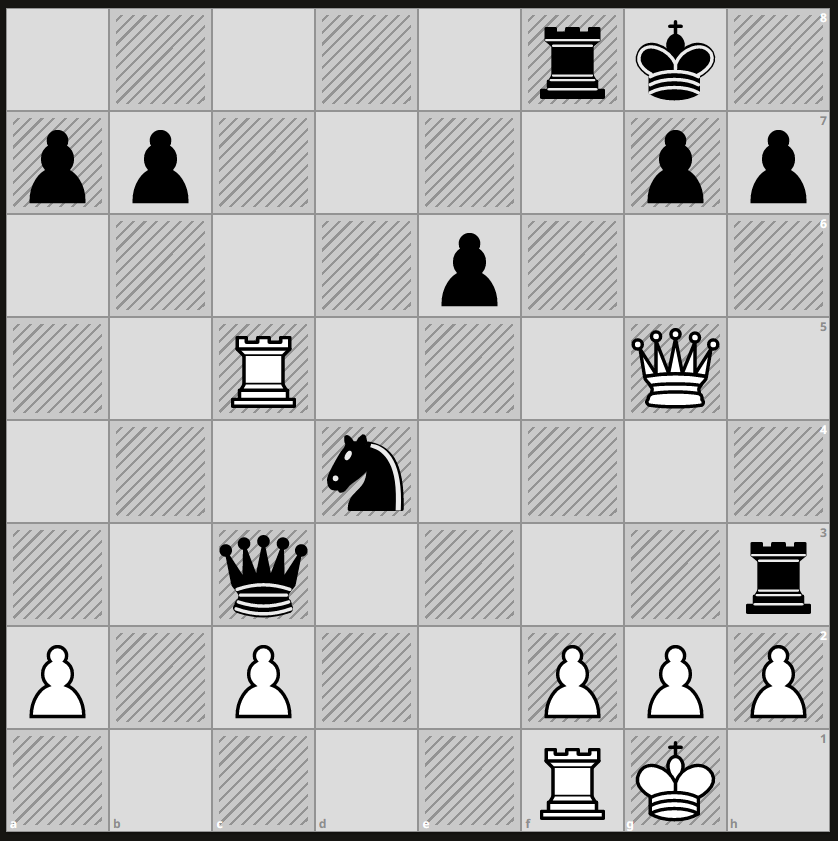
\includegraphics[width=8.0 cm,height=8.0 cm]{marshall-levitsky23.png}
    
\end{center}

En esta posici\'on Marshall, lleva las piezas negras, Levitsky amenaza la dama de Marshall con 23. Tc5 y tratar\'a eventualmente de recuperar el alfil que perdi\'o en h6, pues aún no puede capturar la torre ya que existir\'ia 23. ... Cf3+ y perder\'ia la dama. Aunque en esta posici\'on Marhsall tenía suficientes alternativas para continuar con su ataque, decide hacer una de las jugadas m\'as emblem\'aticas de la historia del ajedrez contemporáneo: 23. ... Dg3.

\begin{center}
    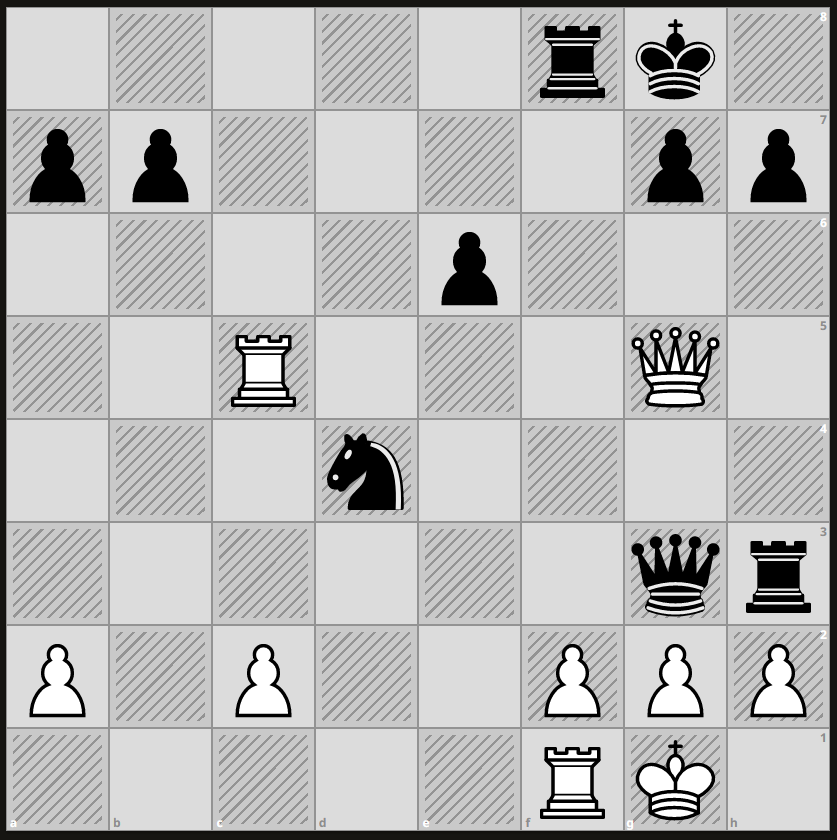
\includegraphics[width=8.0 cm,height=8.0 cm]{marshall-levitsky23-2.png}
\end{center}

Esta jugada es contra-intuitiva, incluso si se es aficionado parece no ser evidente porque se regalar\'ia la dama en esa posici\'on, ya que podría ser capturada por la dama blanca y por los peones de $f$ y de $h$, pero hay que tomar un momento para analizar rápidamente las consecuencias. Si se sigue con 24. Dxg3 negras puede jugar 24. ... Ce2+ 25. Rh8 Cxg3+ y despu\'es de esta secuencia blancas solo puede moverse o capturar el caballo con el pe\'on de $f$. Si lo captura, viene jaque mate con Txf1\#; si no lo captura y juega Rg1, entonces se puede contestar con Cxf1 y la ventaja material para negras ser\'ia suficientemente alta como para que finalice la partida con una victoria, aunque en un tiempo mayor. 

Por otra parte, si se toma la dama con alguno de los peones, las secuencias son similares; si toma con el pe\'on de $h$, viene Ce2\#; si se captura con el pe\'on de $f$, sigue Ce2+ y tras Rh8 se finaliza la partida con Txf1\#. Estas secuencias encantaron al p\'ublico tanto que incluso empezaron a arrojar oro al tablero \cite[p. 138]{marshall2002my} y se le bautiz\'o como \emph{La partida de las monedas de oro}. Es bastante impresionante como Marshall tuvo la creatividad para encontrar la jugada $Dg3$ y lo impresionante que es cómo ésta puede ser capturada de 3 maneras distintas y todas llevan a la derrota.

El aspecto más importante a resaltar --desde una perspectiva propia-- es que si se analiza con módulos más contemporáneos, la partida posee errores y podría estar lejos de ser un juego óptimo de acuerdo a las consideraciones de Zermelo. A pesar de esto, parece haber un consenso de que es una de las partidas más bellas en la historia del juego. Esto detona ciertas consideraciones importantes, pues parecería que el aspecto estético no depende del éxito propio, pues Levitsky aplaudió la gran jugada que hizo Marshall. Tampoco se requiere que la partida se perfecta o que sea adecuada a la estrategia óptima que se sabe que existe. En última instancia ni siquiera es necesario tener la intención de generar belleza en el sistema.

El ajedrez como sistema es capaz de generar secuencias que los humanos dejan de apreciar desde un aspecto formal y pueden otorgarle una apreciación estética que sea regida por criterios ajenos a la lógica. Fenómenos que, como se acaba de mostrar, son similares --en cierto sentido-- a los que ocurren con la matem\'atica. La belleza no est\'a en encontrar la secuencia \'optima o la demostraci\'on de un teorema, sino en el proceso que se sigue para llegar a ello. En la pr\'actica es posible generar secuencias o demostraciones que sean m\'as bellas que otras y desarrollar criterios para discernir c\'omo es que se deben evaluar estos fenómenos, lo cual es una tarea de la est\'etica m\'as que de la l\'ogica.

Obviamente, no es el \'unico an\'alisis est\'etico realizable ni que ya se ha realizado, Johan Huizinga utiliza el ajedrez como fenómeno para ejemplificar unos cuantos aspectos sobre la est\'etica del juego\footnote{Juego de manera general.}. Aunado a esto, hace la siguiente observación sobre el carácter armónico que existe en los juegos:

\begin{quote} \singlespace
 He aqu\'i otro rasgo positivo del juego: crea orden, es orden. Lleva al mundo imperfecto y a la vida confusa una perfecci\'on provisional y limitada. [...] Esta conexi\'on \'intima con aspecto de orden es, acaso, el motivo de por qu\'e el juego, como ya hicimos notar, parece radicar en gran parte dentro del campo est\'etico. \cite[p. 24]{huizinga2020homo},   
\end{quote}


Lo que podr\'ia llevar a un estudio del ajedrez en t\'erminos de armon\'ia u orden, aspecto que tambi\'en se considera en la obra de Montano. Si bien la propuesta de Huizinga no versa particularmente sobre este juego, puede servir para construir un an\'alisis de los torneos, el juego e incluso nutrir la discusi\'on sobre el elitismo intelectual que se ha formado alrededor del ajedrez. 

Esto es solo una breve aproximaci\'on al ajedrez desde una perspectiva est\'etica. Existen a\'un diversas salidas de estudio, pero la relevancia de resaltar estas dos es cómo se pueden enlazar, por una parte, con el proceso de evaluaci\'on que realizan los humanos y, por otra parte, para ofrecer una alternativa al estudio de los torneos que se separe del carácter intelectual que muchas veces les rige y se pueda recuperar un aspecto propiamente l\'udico en lugar de competitivo. Ambas cuestiones sin perder el carácter de ser una discusi\'on de corte filos\'ofico.

\section{El ajedrez como medida intelectual}

\noindent Uno de los fen\'omenos m\'as grandes del ajedrez de todos los tiempos ha sido Robert James Fischer, conocido popularmente como Bobby Fischer. Fue campe\'on mundial durante el periodo de $1972 - 1975$ y hay quienes afirman, sin temor a equivocarse, que el impacto que tuvo Fischer en el ajedrez fue tan significativo como la adici\'on del enroque al juego \cite[p. 219]{golombek1976history}. Existen diversos motivos para realizar estas afirmaciones: en primer lugar, su genio para el ajedrez y, en segundo, el contexto mundial de la \'epoca en la que se volvi\'o campe\'on mundial.

Esta secci\'on se enfoca en el segundo motivo. Hablar acerca del genio ajedrec\'istico de Fischer requerir\'ia una gran cantidad de tiempo y un entendimiento del juego superior al que el texto ha intentado proveer, aunado a ello, la discusi\'on se alejar\'ia del enfoque filos\'ofico que se pretende mostrar. Este enfoque filos\'ofico se encargar\'a de conectar el caso particular del fenómeno Fischer con el an\'alisis de Johan Huizinga sobre el juego\footnote{La concepci\'on de \emph{juego} de Huizinga no es la misma que la de Zermelo.}, pues este lo propone como un fundamento para la cultura: 

\begin{quote}\singlespacing
En esta comparaci\'on no se reconoc\'ia o no se expresaba que el juego y la cultura se hallan, en efecto, implicados el uno en el otro. Ahora se trata de mostrar que el juego aut\'entico, puro, constituye un fundamento y un factor de la cultura. \cite[p. 17]{huizinga2020homo}.
\end{quote}

La intenci\'on de Huizinga es justificar c\'omo es que el juego puede ser un origen de la cultura. Se parte del hecho de que el juego es un fenómeno innato a cualquier ser vivo cuya funci\'on parece ir m\'as all\'a de un rol f\'isico o biol\'ogico: 

\begin{quote}\singlespacing
El juego, en cuanto a tal, traspasa los l\'imites de la ocupaci\'on puramente biol\'ogica o f\'isica. Es una funci\'on ella de sentido. En el juego <<entra en juego>> algo que rebasa el instinto inmediato de conservaci\'on y que da un sentido a la ocupaci\'on vital. \cite[p. 12]{huizinga2020homo}.
\end{quote}

El proceso que sigue consiste en describir c\'omo es que el juego es algo que se observa en los animales y que fundamenta c\'omo esta caracter\'istica puede identificarse en todos los seres humanos. Su intenci\'on es dirigirse a delimitar su estudio, pues tratar de dar una descripci\'on total de lo que es aquel y la din\'amica del mismo en s\'i es una tarea bastante compleja. El objetivo de seguir este proceso es justificarlo como generador de cultura dadas las consecuencias del juego en un entorno social \cite[p. 19]{huizinga2020homo}.

En particular, la propuesta cultural del ajedrez se puede servir de diferentes elementos, aunque se intent\'o proponer un car\'acter est\'etico, de acuerdo con Huizinga, puede ser prescindible y a\'un as\'i el juego tiene potencial como generador de cultura y, eventualmente, un fen\'omeno mucho m\'as amplio:

\begin{quote}\singlespacing Cuando el juego es un bello espect\'aculo, se da, inmediatamente, su valor para la cultura, pero semejante valor est\'etico no es imprescindible para que el juego adquiera car\'acter cultural. Valores f\'isicos, intelectuales, morales o espirituales pueden elevar del mismo modo el juego al plano de la cultura.  \cite[p. 70]{huizinga2020homo}.
\end{quote}

Desarrollar el aspecto cultural del juego partiendo del análisis de Huizinga tiene como propósito mostrar el impacto del juego en la formación cultural y política contemporánea más allá de los aspectos formales y de competencia. Para ello, nos serviremos del caso particular de la figura de Fischer, quien, tras su victoria contra Spassky en 1972, fue aclamado en los Estados Unidos de Norteam\'erica. Se le buscaba como figura para publicidad y deton\'o un inter\'es por el juego que no se hab\'ia visto hasta entonces, se comenta incluso que no hab\'ia tableros de ajedrez disponibles para comprar en algunos lugares de Europa \cite[p. 222]{golombek1976history}\footnote{Una situaci\'on similar surgi\'o tras el estreno de la serie \textit{The Queens Gambit}.}, en gran parte porque una victoria contra los rusos tuvo un impacto m\'as all\'a de lo deportivo.

%%agregar nota sobre capablanca y datos sobre el caso de the queens gamit%%
La Uni\'on Sovi\'etica mantuvo una supremac\'ia ajedrec\'istica que fue consolidada para la \'epoca de los 60's desp\'ues del reinado del cubano José Raúl Capablanca --otro de los grandes genios del ajedrez de todos los tiempos-- . Esta supremac\'ia fue puesta en juego cuando Fischer consigui\'o el derecho a jugar por el t\'itulo mundial y la perdieron --temporalmente-- cuando \'este venci\'o a Spassky en lo que se considera \emph{el match del siglo}, permitiendo que el titulo mundial fuera visto precisamente como un titulo mundial y no como un premio reservado para los jugadores de la URSS \cite[228]{golombek1976history}. En particular la ronda 6 fue aclamada por el p\'ublico y el mismo Spassky --quien se sum\'o a los aplausos del p\'ublico al finalizar la partida-- \cite[p. 225]{golombek1976history}, pues fue una muestra del gran nivel y genio de Fischer, ya que el inicio del enfrentamiento se hab\'ia visto afectado por la inconformidad de Fischer respecto a la sala de juego, el p\'ublico e incluso el equipo sovi\'etico.

Esto tuvo un fuerte impacto pol\'itico. Durante esa \'epoca se estaba desarrollando la \emph{guerra fr\'ia}, un enfrentamiento desarmado entre dos superpotencias, Estados Unidos de Norteam\'erica y la Uni\'on Sovi\'etica \cite[p. ix]{mason2002cold}. Mientras el ajedrez ganaba popularidad y el juego pas\'o a ser deporte, se empez\'o a generar una cultura alrededor de \'el. Esto puede verse reflejado en sus jugadores y en la din\'amica de los torneos. A diferencia del resto de deportes, el ajedrez de \'elite se jugaba vestido de traje, el tiempo se med\'ia con relojes mec\'anicos para cada mesa, la puntualidad era un elemento fundamental y se desarroll\'o una etiqueta durante el juego. Aspectos como dar la mano al oponente al iniciar una partida y ante una victoria o derrota, o el simple hecho de respetar reglas que obligaban al jugador a mover la primera pieza que hab\'ia tocado hac\'ia que el ajedrez tuviera un sello diferente al del resto de deportes. La competencia no era f\'isica, sino intelectual.

Esta situaci\'on fue reconocida por ambos gobiernos, pues era un secreto a voces que Rusia y Estados Unidos de Norteam\'erica se encontraban en este enfrentamiento por la oportunidad de medir la supremacia de sus ideales, contrastando el individualismo americano en contra de los ideales del r\'egimen socialista:

\begin{quote} \singlespace
    Las reacciones de ambos bandos fueron extremas. Los soviéticos consideraron la derrota de Spassky como una derrota nacional. Los estadounidenses aclamaron a Fischer como un héroe. El presidente Richard Nixon le envió un telegrama de felicitación y una invitación a la Casa Blanca.Tras su gran éxito, Bobby Fischer desapareció de la vida pública durante más de 20 años. Nunca volvió a jugar un partido oficial por puntos de clasificación. \cite{guerrafria_fischerspassky}
\end{quote}


Para ese momento se ha generado una cultura no de qui\'en es el m\'as fuerte, sino de qui\'en es el m\'as listo, lo cu\'al resulta mucho m\'as relevante para el conflicto debido a que, dada la personalidad de Fischer, el enfrentamiento contra Spassky fue mostrado como un duelo de un hombre contra toda la Uni\'on Sovi\'etica\footnote{El individualismo estadounidense.}. Los sovi\'eticos eran estigmatizados --probablemente gracias al régimen socialista-- como personas que siempre trabajaban en equipo, hasta cuando la competencia era de manera individual. Esto foment\'o que la derrota de Spassky se sintiera a\'un m\'as fuerte, pues Fischer no lo habr\'ia derrotado solo a \'el, sino a todo su equipo y, desde una perspectiva m\'as extravagante, a toda la Uni\'on Sovi\'etica. Por supuesto, esta victoria no mostraba la fuerza bruta, sino que representaba a los estadounidenses como una comunidad que posee una inteligencia superior comparada con la URSS. Esta búsqueda por una superioridad intelectual puede verse reforzada con sus esfuerzos por ganar tanto en la carrera armament\'istica como en la carrera espacial \cite[p. 15]{millan2012guerra}.

La estancia de Fischer en la cima no duraría tanto a pesar de su éxito. Su estado mental se deterioró rápidamente durante su preparación contra Spassky y para el momento de la revancha parecía encontrarse temeroso de perder. Esto lo llevó a pedir condiciones muy inclinadas a su favor para la revancha por el título: 

\begin{quote} \singlespace
    [...] el número de juegos debe ser ilimitado y, en caso de que en el juego se alcance una puntuación de $9-9$ debe ser considerado como un empate y el campeón actual retendría el título \cite[p. 235]{golombek1976history}.
\end{quote}

Esto lo llevó a discutir constantemente con la FIDE, gracias a ello les comunicó que no participaría en la defensa por el título, situación que rechazó la FIDE y le invitaron a reconsiderar su postura, a lo que Fischer nunca contestó y desapareci\'o de la escena profesional\footnote{Debido a exigencia excesiva sobre Fischer.}. Gracias a esto se designó como campeón al candidato que había obtenido el derecho a competir por el título, Anatoly Karpov\footnote{Por lo mismo, Karpov es el único campeón del mundo que nunca ganó una partida contra otro campeón mundial.}. Esta situación permite que los soviéticos --eventualmente rusos-- recuperen el título mundial, al menos hasta el 2000 con Alexander Khalifman. En este periodo post-Fischer se enfrentaron dos jugadores que a día de hoy siguen siendo reconocidos como verdaderos genios, tanto en el ámbito ajedrecístico como fuera de él: Garry Kasparov y Anatoly Karpov.

Ya se ha hablado sobre Kasparov en una sección anterior. Fue campeón mundial tanto de la FIDE como de la PCA\footnote{Una asociación de ajedrecistas creada por el dados ciertos descontentos de Kasparov con la FIDE.} y uno de los duelos más relevantes de su carrera fue contra Deep Blue, el computador de IBM que comenzó la superioridad de las maquinas en el ajedrez ante los seres humanos. Si bien estos algoritmos al día de hoy no son infalibles --al menos para el ajedrez, gracias a la prueba de Zermelo-- sí son mucho más eficientes que los humanos dada la cantidad de posiciones que evalúan y la manera de discernir entre cuál es la mejor jugada. En el caso de estudio de las damas se mostró como es que se utilizan bases de datos de finales y de aperturas para que a lo largo del juego, de llegar a una posición conocida, se pueda acceder a la secuencia óptima y ejecutarla para finalizar el juego. Este proceso se ha ido optimizando con el pasar de los años para casos particulares, como las damas o el ajedrez. El resultado es que hoy en día los módulos poseen algoritmos que pueden vencer a los mejores jugadores del mundo en casi la totalidad de las veces. Si el objetivo absoluto del ajedrez fuera ganar, la competencia se hubiera centrado en las herramientas tecnológicas y su óptimo desarrollo, pero en lugar de eso, el aspecto cultural y lúdico que se había gestado durante tantos años alrededor el juego permitió que, en lugar de desaparecer el ajedrez, los humanos aprovecharan esas herramientas.

Retomando nuestra tesis principal y sabiendo que las computadoras se volvieron imbatibles para los humanos --en parte gracias a Zermelo-- podr\'ia pensarse que el ajedrez desaparecer\'ia, pero los humanos no desperdiciaron la oportunidad de utilizarla como herramienta de entrenamiento o preparación. En la actualidad, un ajedrecista profesional\footnote{Se entenderá por profesional a aquél jugador que juega de manera competitiva y depende económicamente del deporte.} --y cualquiera en realidad-- puede utilizar estas herramientas tecnológicas, como bases de datos, ya sea para aperturas, finales o celadas. Esto se debe a que los ordenadores --como se mostró en el capítulo (2.1.2)-- pueden volver eficiente el proceso de cálculo al enlazar la partida en turno con algún final ya conocido y si esta información es accesible para los humanos, se pueden reconocer posiciones y el resultado que se puede forzar.

Además de utilizar las bases de datos, es posible también servirse de estos modelos para evaluar posiciones, dado que se puede llevar el registro de las partidas, tras un torneo siempre es posible escribirle la secuencia a un módulo y que éste arroje las mejores respuestas de cada jugador o revelar si existe alguna secuencia que no se observó durante la partida y que pudo haber cambiado el resultado. El desarrollo tecnológico tanto de módulos como el crecimiento de las bases de datos ofrece una cantidad de herramientas enorme, la cual también permite que los jugadores actuales se desarrollen de manera más rápida y ha generado un mayor acceso al juego de alto nivel, pues ya no es indispensable una academia o un entrenador personal. El ajedrez y la cultura alrededor de \'el lejos de verse mermado por la tecnolog\'ia se ha enriquecido y ha permitido un mayor acceso al juego.

Por supuesto, como cualquier herramienta tecnológica, \'esta es un arma de doble filo y el ajedrez no se ha visto libre de trampas auxiliadas por la tecnología. No está prohibido que los jugadores aprovechen las herramientas tecnológicas para prepararse, estudiar e incluso estudiar a sus rivales, pero estas herramientas deberían estar limitadas al entrenamiento. De usar las herramientas tecnol\'ogicas en la pr\'actica, el deporte ya no ser\'ia una competencia entre humanos, sino entre m\'odulos o en \'ultima instancia, no s\'olo que m\'odulo es m\'as eficiente, sino que dispositivo portátil puede resolver una secuencia de manera m\'as r\'apida, es decir, si se permite que el uso de la tecnología se vuelva parte de las competencias entre humanos --y no solo del entrenamiento-- el juego se volvería trivial, la competencia sería para ver quien tiene el mejor o más eficiente algoritmo y eso eventualmente generaría un declive del ajedrez como deporte y una eventual pérdida de la cultura.

Por eso mismo, cuando hay una compensaci\'on econ\'omica de por medio, algunos jugadores est\'an dispuestos a dejar de lado tanto la \'etica deportiva como su propia \'etica. Existen diversas aplicaciones de ajedrez que hoy en d\'ia cuentan con un motor que, en sus niveles m\'as altos, es imbatible incluso para los mejores jugadores del mundo. Esto ha llevado a que diversos jugadores los utilicen para hacer trampa. En 2015, en el torneo Abierto de Dubai el gran maestro Gaioz Nigalidze fue de manera repetida al sanitario durante la ronda 6 contra Tigran Petrosian. Tanto a este jugador como al árbitro les llam\'o la atenci\'on la gran cantidad de veces que ten\'ia que ir, adem\'as de que siempre iba al mismo ba\~no, a\'un habiendo m\'as cubículos disponibles. Esto llev\'o a que se examinara el lugar y se descubriera un tel\'efono movil con los datos de la partida en turno, lo que lo llev\'o a una suspensi\'on del torneo y a una suspensi\'on de los torneos oficiales de la FIDE \cite{gm_haciendotrampa}.

Las trampas auxiliadas por la tecnolog\'ia se volvieron incluso m\'as recurrentes dado el incremento de torneos y eventos en linea durante el periodo $2019 - 2022$, ya que al jugar desde casa la posibilidad de recibir ayuda externa se volv\'ia enorme. Para solucionar este tipo de problemas hubo propuestas como transmitir audio y video del cuarto en el que los jugadores se encontraban. A pesar de esto, hubo personas que se mantuvieron haciendo trampa, como es el caso de Hans Niemann, un joven prodigio de 19 años.

Niemann ha confesado haber hecho trampa en juegos en línea auxiliandose de herramientas tecnológicas en más de una ocasión:

\begin{quote} \singlespace
    Hice trampa en partidas aleatorias en Chess.com, pero lo confesé. Fue el error más grande de mi vida. Y estoy completamente avergonzado. Se lo digo al mundo porque no quiero tergiversaciones. Nunca he hecho trampa en un juego sobre el tablero. Y aparte de cuando tenía 12 años, nunca hice trampa en un torneo con premios en metálico. \cite{marca_niemann_trampa}
\end{quote}

El caso de Niemann es particularmente interesante por dos motivos: el primero es que en septiembre de 2022 se abrió una controversia entre él y el entonces campeón del mundo Magnus Carlsen dado que el joven estadounidense lo venció en la tercera ronda. Tras esta situación Carlsen abandonó el torneo y declaró que sospechaba que Niemann había estado haciendo trampa. La segunda es que una de las justificaciones que tenía Carlsen para acusarlo de ello fue el comportamiento que tuvo durante la partida, en palabras de Carlsen: 

\begin{quote}\singlespace
    Magnus Carlsen [MagnusCarlsen]. \citeyear{comunicado_carlsen}
    
    Creo que Niemann ha hecho trampa más --y más recientemente-- de lo que ha admitido públicamente. Su progreso sobre el tablero ha sido inusual, y a lo largo de nuestro juego en la Copa Sinquefield tuve la impresión de que él no estaba tenso o incluso completamente concentrado en el juego en posiciones críticas, mientras me jugaba mejor con negras de un modo que yo pienso solo un puñado de jugadores pueden hacer. [Tweet]. Recuperado de \url{https://twitter.com/MagnusCarlsen/status/1574482694406565888}
\end{quote}

Esto abre por supuesto otros aspectos del ajedrez en su carácter deportivo. A pesar de parecer un deporte no tan demandante físicamente, tanto las afirmaciones de Carlsen como el agotamiento mental que experimentan los jugadores después de partidas clásicas, parecen evidenciar que la exigencia física del ajedrez es superior a la que pareciera. De hecho puede ser un factor determinante tanto en el desempeño de un jugador como en la percepción del rival sobre éste mismo. Y retomando la idea anterior, si esto se permitiera, el ajedrez probablemente perder\'ia todo su sentido. 

El caso escaló tanto de nivel --en parte gracias a los antecedentes de Niemann-- que se realizó una investigación exhaustiva sobre su caso y, a pesar de no haber encontrado evidencia de que utilizara la ayuda ya sea de alguien externo o de un recurso tecnológico, la sospecha de que hacía trampa siguió creciendo gracias a que se analizaron varias de sus partidas y se encontr\'o que algunas rozaban una precisión absoluta. Esta situaci\'on no suele ser rara en jugadores de élite pero solo en las primeras jugadas o momentos cr\'iticos de una partida, mientras que Niemann consiguió finalizar realizando movimientos de módulo en al menos 10 partidas en diferentes eventos, lo que parece sobrehumano\footnote{Esto de acuerdo con la evaluación de módulos de ajedrez. Este tipo de evaluaciones se pueden hacer gracias a las aportaciones de Zermelo sobre la estrategia óptima, por lo que incluso en las discusiones éticas sobre el juego, sigue presente el aporte de Zermelo.} \cite{hansniemannnumbers}.

Esto mantuvo y elevó las sospechas de que utilizaba un dispositivo para comunicarse. Hubo gente que incluso se atrevió a decir que el dispositivo se encontraba dentro de su cuerpo y emitía vibraciones para indicarle el movimiento a realizar. Durante muchos eventos de élite es común que a los jugadores se les escanee con un detector de metales para prevenir que se ingrese con un celular o dispositivo electrónico a la sala de juego. El rumor sobre Niemann fue tan fuerte que en un evento de este tipo se observa como incluso se le escanea de manera más exhaustiva que al resto de jugadores.

El caso de Niemann muestra varias cosas relevantes sobre el ajedrez como deporte y sus jugadores. De nuevo hay una exposición sobre su carácter de élite intelectual, pues las acusaciones en su contra no hubieran tenido tanto alcance si no fueran por parte de Magnus Carlsen. Aunado a esto, se puede observar como incluso los jugadores de élite reconocen la superioridad de los computadores contra los humanos, pues parece que el tener acceso a estas herramientas durante una competencia vuelven al jugador imbatible, como se había dicho. Esta misma superioridad de los módulos sobre los jugadores fue consolidada cuando Kasparov fue vencido por Deeper Blue. Con el paso del tiempo esta brecha de nivel en el juego no ha hecho más que crecer y probablemente así seguirá.

El genio de Kasparov no sólo se mantuvo en el ámbito ajedrecístico, además su derrota contra Deep Blue no lo limitó para seguir compitiendo de manera profesional. Junto a su carrera en el ajedrez --y posterior a esta-- se adentró en el mundo de la política. De manera contemporánea se le conoce popularmente como un opositor de Vladimir Putin y --según Kasparov-- de cualquiera que atente contra el mundo libre. En 2016 fue invitado a una plática por parte del Carnegie Council en donde se habla de su inseguridad respecto a Rusia y presenta uno de sus libros que no versa sobre el ajedrez: \textit{Winter is Coming: why Vladimir Putin and the enemies of the free world must be stopped} \citeyear{kasparov2015winter}.

\begin{quote} \singlespace
    Lo que es menos conocido sobre él es que en la década pasada ha tenido una segunda carrera en política ``haciendo frente a la creciente ola de represión'' viniendo del Kremlin. Estuvo activo en las marchas anti-Putin hasta que una implacable represión redujo la oposición abierta. Después de desafiar una elección presidencial a Putin en 2007, una que fue descalificada bajo circunstancias turbias y una serie de lo que él llama ``accidentes'', ya no se sentía seguro viviendo en Rusia. Temiendo que le quitaran su pasaporte ruso, se exilió en el extranjero. \cite{winter_is_coming}
\end{quote}

En su libro \'el mismo habla de la situaci\'on del mundo actual o al menos de cómo la percibe. Un aspecto interesante de observar es que uno podr\'ia preguntarse por qu\'e Kasparov siendo un genio en el ajedrez sea tan influyente en el aspecto político. Tras observar el fen\'omeno de Fischer se puede notar que el ajedrez otorga un estatus superior --tanto intelectual como social-- a aquellos que se destacan en el deporte, por lo que sirve como gran respaldo a la hora de iniciar la carrera pol\'itica de Kasparov sobre todo en Rusia, donde el juego tiene una cantidad enorme de adeptos que le ven seriedad y profesionalismo. Queda en cuestión si el ser sobresaliente en el ajedrez es suficiente respaldo para considerar que si una persona es excelente en el deporte, puede serlo en otros ámbitos tan distintos.

Adem\'as de su incursi\'on en la pol\'itica, Kasparov se ha convertido en uno de los m\'as grandes impulsores del ajedrez en el mundo contempor\'aneo, personalidades como Leontxo Garc\'ia --otro gran periodista del deporte-- lo considera el mejor jugador de todos los tiempos, no particularmente por su nivel como jugador, sino por sus contribuciones y difusión del ajedrez. La Fundación Kasparov de Ajedrez para Iberoamérica es uno de los proyectos con los que busca difundir el ajedrez en el continente. Gracias a esta fundación se han podido realizar eventos como el Gran Encuentro con el Ajedrez Educativo UNAM 2016, que contó con el estreno de una película, una cantidad enorme de ponencias referente al juego, un torneo cerrado para la \'elite iberoamericana y un torneo abierto para todo el público.

La relevancia del ajedrez como competencia no est\'a limitada al campeonato del mundo, pues tambi\'en existen distintos eventos que buscan promover la profesionalizaci\'on del deporte. Entre ellos se encuentra la Olimpiada de ajedrez, que es un torneo por equipos que se ha celebrado desde 1927, ocurre cada dos años y tiene la participación de una gran cantidad de países de todo el mundo. Esta olimpiada tiene un gran peso a la hora de exhibir el nivel deportivo de varios países, pues mientras el equipo noruego --que posee al anterior campeón del mundo-- no ha tenido participaciones destacadas en las últimas justas, pa\'ises como Rusia exhiben su superioridad llevado equipos a la olimpiada de ajedrez tan fuertes que pose\'ian a varios campeones del mundo \cite{cinco_campeones}.

A pesar de esto, no ha sido posible que el ajedrez sea incluido en los juegos olímpicos como una disciplina más. Para las Olimpiadas de París 2024 la FIDE redactó una carta donde se solicitaba que el ajedrez fuera una más de las disciplinas a disputar, argumentado los motivos por los cuáles podía ser parte de los juegos olímpicos, sin embargo esta solicitud fue rechazada \cite{olimpicos_sinajedrez}. Una de las razones aparentes es que no en todos los países se le considera un deporte dado que parece no requerir un esfuerzo físico de la misma magnitud que si lo requieren otros deportes, pues mientras que se aceptó añadir disciplinas como la escalada o el skateboarding, el ajedrez sigue sin encontrar un lugar en los juegos olímpicos. Por supuesto, queda en cuestión si esta es la verdadera razón o si existe algo más, pues hay que considerar que si se añade el ajedrez como disciplina, podría convertirse en el primer deporte \emph{intelectual} en ser reconocido, lo que probablemente abriría camino a disciplinas como el Go, juegos electrónicos de estrategia como Dota, League of Legends, Starcraft o Clash Royal que pueden contrastar con lo que generalmente se concibe como deporte.

Esto es otra muestra del aspecto cultural y privilegiado que posee el ajedrez. No es raro encontrar jugadores que migren --aunque sea de manera temporal-- del ajedrez a algún videojuego de estrategia, como fue el caso de Ian Nepomniachtchi, el actual subcampeón mundial. Durante una época de su vida dejó momentáneamente el ajedrez y se dedicó a jugar Dota, volviéndose jugador semiprofesional y ganando un par de torneos junto a su equipo. A pesar de ello, este evento en su vida no resulta muy relevante, pues la cultura construida alrededor del ajedrez no se puede ver opacada por el reciente surgimiento de otras disciplinas, como los deportes electrónicos.

Mientras que un jugador de ajedrez puede incluso ser catalogado como un genio --como Kasparov o Fischer-- y ser categorizado como una persona elegante o culta --entre otras cosas--, un jugador de, por ejemplo, Starcraft, parece no tener el mismo derecho, a pesar de seguir siendo una competencia intelectual. Esto se debe a una mera cuestión cultural, pues en países con un régimen y estilo de vida diferente al occidental se está construyendo una cultura alrededor de este tipo de videojuegos. Tal es el caso de League of Legends en Corea del Sur, que está en proceso de generar una propia cultura alrededor de él, tal como lo empezó a hacer el ajedrez en occidente hace unos años.

El impacto es tan grande que en los Juegos Asiáticos de 2023 el equipo surcoreano consiguió la presea de oro en la competencia de League of Legends, lo que les mereció tanto el reconocimiento del gobierno como la exención del servicio militar surcoreano \cite{juegosasiaticos}. Esto es de suma importancia, ya que en este país el servicio militar es obligatorio para todos los hombres y no cumplir con el antes de los 28 años es causa de prisión\footnote{Ni siquiera los grupos musicales más importantes de Corea del Sur han tenido tal privilegio, hasta ahora son primordialmente deportistas, a pesar de que la industria del entretenimiento introduce un gran capital económico.}. El juego se encuentra generando una cultura que para la actualidad tiene un impacto político, pues figuras como la de Lee Sang Hyeok, conocido como \emph{Faker}, se han vuelto tan relevantes para su gobierno que podría compararse incluso con la importancia que tuvo Fischer en su momento para los Estados Unidos de Norteamérica. A pesar de esto, sigue sin ser claro por qué el ajedrez y su aspecto cultural le siguen otorgando un aspecto privilegiado. Puede ser en parte porque los jugadores de esports no tienen el mismo caracter intelectual o elegante del ajedrez, pero eso no garantiza que algún otro fenómeno no se pueda hacer de una cultura similar, como de hecho ya está pasando en oriente.

Parece m\'as evidente entonces c\'omo es que a trav\'es del juego surge una cultura que puede tener diferentes repercusiones. El fen\'omeno Fischer junto con personalidades como Kasparov consolidaron a la cultura del ajedrez como una competencia intelectual, no particularmente por su genio, sino por el contexto alrededor de \'el y las áreas en las que se desempeñaron. El ajedrez ya hac\'ia tiempo que dej\'o de ser solo un juego, ya se hab\'ia generado una cultura alrededor de \'el y, sin embargo, el an\'alisis no se agota ah\'i. La teor\'ia de Huizinga permite analizar c\'omo es el surgimiento de una cultura a trav\'es del juego --esta vez, en el sentido coloquial de la palabra-- y deja el camino abierto para observar sus consecuencias, en este caso, \'eticas y pol\'iticas m\'as all\'a de lo que nos puede decir el an\'alisis l\'ogico y formal del juego.

\section{Conclusiones}

Como se ha podido observar, el ajedrez como fenómeno puede ser objeto de estudio a trav\'es de distintas \'areas. No es necesario ni indispensable que se le aborde desde la l\'ogica para propiciar un an\'alisis de corte filos\'ofico. Su exposici\'on como juego basta para que se le dé una perspectiva desde la est\'etica, su complejidad en terminos de c\'omputo puede ponerlo a ojos de la epistemolog\'ia y la matem\'atica y su panorama hist\'orico parece ser suficientemente amplio como para estudiar las consecuencias pol\'iticas del mismo y el estatus que el mismo juego cre\'o para si mismo y para sus jugadores.

Cada uno de estos an\'alisis puede extenderse tanto como se desee, no son los \'unicos en sus \'areas y tampoco son las \'unicas \'areas disponibles, pero ahondar en cada uno de ellos requerir\'ia una dedicaci\'on al menos similar a la que se le di\'o al estudio desde la perspectiva conjuntista. A pesar de esto, es importante resaltar que la teor\'ia y los aportes de Zermelo se mantienen de fondo en estas distintas perspectivas. En el aspecto epist\'emico gracias a Zermelo se puede inferir que la complejidad es tan alta para los humanos y las máquinas que les resulta imposible procesar toda la informaci\'on del juego. Esto deriva en el aspecto est\'etico y la búsqueda de alternativas como objetivo en el ajedrez que no necesariamente dependan de la victoria. Finalmente, sigue presente en la constituci\'on del juego como fen\'omeno cultural y el perfil intelectual de sus jugadores, lo que ha llegado a tener repercusiones de car\'acter pol\'itico.

El hacer esta breve introducci\'on pretende mostrar que, incluso si el ajedrez en terminos l\'ogicos no es filos\'oficamente relevante, puede serlo en t\'erminos epist\'emicos. Si no es relevante en t\'erminos epist\'emicos, puede serlo en t\'erminos est\'eticos. Si no parece relevante incluso en t\'erminos est\'eticos, a\'un puede serlo en t\'erminos pol\'iticos y culturales. El que sea posible abordarle desde diversas \'areas de la filosof\'ia puede servir como justificaci\'on para exhibir que el ajedrez de hecho es un fen\'omeno filos\'oficamente interesante y espero haber mostrado que, en efecto, es un fenómeno filos\'oficamente relevante.


\chapter*{Conclusión}
\addcontentsline{toc}{chapter}{Conclusi\'on} 

El objetivo principal del trabajo consist\'ia en exhibir c\'omo es que a pesar de que el teorema de Zermelo muestra que el ajedrez est\'a determinado y que existe una estrategia \'optima, esto no perme\'o de manera significativa la pr\'actica del ajedrez. A lo largo del primer cap\'itulo se realiz\'o una breve introducci\'on hist\'orica a la vida de Ernst Zermelo y al panorama hist\'orico general del teorema para introducir al lector a la discusi\'on. Despu\'es se realiz\'o una reconstrucci\'on del teorema original con la intenci\'on de que fuera m\'as accesible su lectura tanto por el idioma como por la complejidad que puede representar interpretar la maquinaria conjuntista. Esta secci\'on representa el n\'ucleo del trabajo, pues poder analizar con mayor profundidad el teorema de Zermelo permite intentar responder a las preguntas que detonaron la tesis.

Para ello, se hizo el esfuerzo de acotar el teorema --sin perdida de generalidad-- al ajedrez, lo que permite exhibir que tanto crece el juego en t\'erminos de posiciones y complejidad de c\'omputo, para que fuera posible hacer una comparaci\'on con otros sistemas. Esta comparaci\'on se realiz\'o en un segundo capitulo que muestra como para diferentes sistemas regidos por el teorema, el encontrar tanto la estrategia \'optima como el resultado del juego pasa de ser trivial a una tarea que puede llevar a\~nos de trabajo --e incluso puede considerarse incompleta-- y despu\'es a un trabajo que, a pesar de ser computable, la tarea ser\'ia tan larga que simplemente resulta imposible de llevar a cabo.

Estas consecuencias permiten determinar que en efecto, la pr\'actica del ajedrez no ha sido afectada sustancialmente a pesar del teorema de Zermelo, esto se debe a que la complejidad de resolver el juego siguiendo el proceso descrito en el teorema es muy elevada, pues para obtener el algoritmo tendría que aplicarse el análisis regresivo a cada final posible. Esto abre por supuesto varias preguntas sobre el juego, como qu\'e hacen los humanos si el proceso es irresoluble. Esta pregunta se abord\'o de varias maneras, todas ellas como una introducci\'on a otras formas de realizar un an\'alisis filos\'ofico del ajedrez desde diferentes \'areas de la filosof\'ia.

Mientras que la epistemolog\'ia ofrece una alternativa para diferenciar los procesos cognitivos de los humanos contra el c\'aclulo en bruto de las máquinas, o discutir si en realidad el ajedrez puede ser una medida de inteligencia entre humanos y máquinas. La est\'etica ofrece otras perspectivas de estudio, que van desde su car\'acter arm\'onico similar al de las matem\'aticas hasta una belleza que se puede apreciar s\'olo si se tiene un entendimiento del juego que permita entender una posici\'on o secuencia. Por \'ultimo se intent\'o mostrar que aparte de estos acercamientos existen formas pol\'iticas y culturales de abordar el juego que pueden conectarse directamente con el aspecto epist\'emico, pues una parte de la controversia de Niemann se debe a que su juego --en ocasiones-- se parece m\'as al de una maquina que al de un humano, situaci\'on que parece opuesta al enfrentamiento entre Kasparov, donde Deep Blue dio la finta de haber sido intervenida por un humano, por lo que se abren diversas rutas para discutir filos\'oficamente al ajedrez.

Estas aproximaciones mostraron que si bien la pr\'actica del ajedrez no se vi\'o modificada directamente por el teorema de Zermelo, si existen diversos aspectos relacionados con el teorema que si la han modificado. Saber que los ordenadores procesan el juego de diferente manera a los humanos puede hacer que se busque una medida diferente para evaluar la comparaci\'on entre la inteligencia de los seres humanos a lo que se concibe como \emph{inteligencia artificial}. Conocer los factores que rigen la belleza del juego pueden guiar una partida, un estilo de aprendizaje e incluso la intencionalidad, pudiendo poner en primer lugar la búsqueda de una secuencia con propiedades est\'eticas en lugar de una victoria.

Del mismo modo, la pol\'itica y la \'etica pueden modificar c\'omo se juega y c\'omo se practica el juego, como pas\'o en la Uni\'on Sovi\'etica en contraste con c\'omo se desarrollaba el ajedrez en Estados Unidos de Norteam\'erica. Por lo tanto, mientras que el teorema de Zermelo y el an\'alisis conjuntista no modificaron de manera significativa la pr\'actica del ajedrez, sí aportaron demasiada informaci\'on sobre el juego, sobre la complejidad para resolverlo y sobre c\'omo volver computable el proceso. La pr\'actica, por otro lado, puede verse mayormente afectada por otras \'areas en las que espero poder profundizar en un trabajo posterior. 

\chapter*{Bibliografía}

\addcontentsline{toc}{chapter}{Bibliografía}
\bibliographystyle{apacite}
\bibliography{ref}

\end{document}